\documentclass[11pt]{article}
\usepackage[margin=1in]{geometry}
\usepackage{graphicx}
\usepackage{amsmath}
\usepackage{amssymb}
\usepackage{xcolor}
\usepackage{caption}
\usepackage{array}     % needed for !{...} column separators
\usepackage{booktabs}
\usepackage{placeins}
\usepackage[hidelinks]{hyperref}

\graphicspath{{figs/}}
\newcommand{\mpanel}[1]{\includegraphics[width=0.31\linewidth]{#1}}

\title{Results --- revised submission --- original style}
\author{}
\date{}

\begin{document}
\maketitle

\section{Datasets}

\begin{table}[!htbp]
\centering
\begin{tabular}{l|l|r|r|r|r|r}
\hline
\# & Name & $N$ & $P$ & $K$ & MeanIR & CVIR \\
\hline
1  & GpositivePseAAC & 519  & 440  & 4  & 3.86  & 1.15 \\
2  & VirusPseAAC     & 207  & 440  & 6  & 8.62  & 0.92 \\
3  & CHD\_49         & 555  & 49   & 6  & 5.77  & 1.60 \\
4  & Emotions        & 593  & 72   & 6  & 1.48  & 0.16 \\
5  & Scene           & 2407 & 294  & 6  & 1.25  & 0.11 \\
6  & PlantPseAAC     & 978  & 440  & 12 & 6.69  & 0.68 \\
7  & Water-quality   & 1060 & 16   & 14 & 1.77  & 0.29 \\
8  & Yeast           & 2417 & 103  & 14 & 7.20  & 1.82 \\
9  & HumanPseAAC     & 3106 & 440  & 14 & 15.29 & 1.05 \\
10 & enron           & 1702 & 1001 & 53 & 10.45 & 0.80 \\
\hline
\end{tabular}
\caption{(Table 3) Datasets used in the revised experiments. $N$, $P$, $K$ are the number of instances, features, labels. MeanIR and CVIR report per-label imbalance (higher = more imbalanced).}
\label{tab:datasets_revised}
\end{table}

\section*{Pending follow-ups (to fill before final submission)}
\begin{itemize}
  \item \textbf{LGBM run on \texttt{enron}.} Sequentially training (~2--3h
        per task due to K=53 pairwise classifiers); will be merged into
        \texttt{full\_enron\_split\_lgbm\_summary/} when complete and the
        LGBM aggregate panels regenerated.
  \item \textbf{Extended PartialAbstention metrics.} The evaluator has been
        extended with 11 new PA metrics
        (\texttt{jaccard\_pa}, \texttt{\{example,macro,micro\}\_\{precision,recall,f1\}\_pa},
        \texttt{mfrd\_pa}, \texttt{afrd\_pa}). Existing runs were summarised
        with the previous metric set; the new columns will populate
        automatically on the next end-to-end training+evaluation pass.
\end{itemize}


\section{Method encoding}\label{sec:method_encoding}
For every panel that follows, the x-axis encodes the classifier as one of
12 methods, grouped into three blocks:

\paragraph{Block A --- Order-based predictors (ours, indices 1--8).}
Each name has the form \texttt{<order>-<target>-<height>}:
\emph{order} $\in$ \{PA = partial order, PR = pre-order\};
\emph{target} $\in$ \{H = Hamming, S = Subset~0/1\};
\emph{height} $\in$ \{2, $\infty$ (omitted in the label)\}.
\begin{itemize}
  \item 1\,=\,\textbf{PA-H-2}: partial order, Hamming target, height $\le 2$.
  \item 2\,=\,\textbf{PA-H}: partial order, Hamming target, unrestricted height.
  \item 3\,=\,\textbf{PA-S-2}: partial order, Subset 0/1 target, height $\le 2$.
  \item 4\,=\,\textbf{PA-S}: partial order, Subset 0/1, unrestricted.
  \item 5\,=\,\textbf{PR-H-2}: pre-order, Hamming, height $\le 2$.
  \item 6\,=\,\textbf{PR-H}: pre-order, Hamming, unrestricted.
  \item 7\,=\,\textbf{PR-S-2}: pre-order, Subset 0/1, height $\le 2$.
  \item 8\,=\,\textbf{PR-S}: pre-order, Subset 0/1, unrestricted.
\end{itemize}

\paragraph{Block B --- Standard MLC baselines from the original paper
(indices 9--11).}
\begin{itemize}
  \item 9\,=\,\textbf{BR} (Binary Relevance): $K$ independent binary
        classifiers, one per label.
  \item 10\,=\,\textbf{CC} (Classifier Chain): sequential chain that uses
        previous labels as features.
  \item 11\,=\,\textbf{CLR} (Calibrated Label Ranking): pairwise label
        ranking with a calibration label that separates relevant from
        irrelevant.
\end{itemize}

\paragraph{Block C --- Extended baseline added for the revision
(index 12).}
\begin{itemize}
  \item 12\,=\,\textbf{ECC} (Ensemble of Classifier Chains): averages over
        multiple CCs with random chain orders.
\end{itemize}

\paragraph{Reading the panels.} Each panel plots one dotted line with
markers per noise level, colored as in the original paper's Table~5:
\textcolor{red}{$\alpha=0.0$}, \textcolor{blue}{$\alpha=0.1$},
\textcolor{green!60!black}{$\alpha=0.2$}, \textcolor{black}{$\alpha=0.3$}.
\emph{PartialAbstention} and \emph{ScoreVector} panels show only indices
1--8 (the remaining baselines do not export a partial-abstention prediction
nor a probabilistic score vector). Vertical dashed lines at $x=4.5$,
$x=8.5$, and $x=11.5$ separate the four method groups: PA (1--4), PR
(5--8), standard baselines BR/CC/CLR (9--11), and ECC (12). Missing methods show as gaps in the line (with a small grey
``x'' on the axis when the method has no data at all for that panel).

\clearpage

\section{Paper results (RF base learner)}

Reproduces the layout of the original paper's main experiment tables (Tables~5--7): 3 datasets across, 4 metrics down, one table per prediction type (binary vector, partial abstention, score vector). Per the revision, $f^{\mathrm{ham}}_{\mathrm{MLC}}$ and $f^{\mathrm{sub}}_{\mathrm{MLC}}$ are dropped in favour of $f^{\mathrm{Jacc}}_{\mathrm{MLC}}$.


\pdfbookmark[2]{Table 3: Datasets}{paper-rf-datasets}

\begin{table}[!htbp]
\centering
\begin{tabular}{l|l|r|r|r|r|r}
\hline
\# & Name & $N$ & $P$ & $K$ & MeanIR & CVIR \\
\hline
1  & GpositivePseAAC & 519  & 440  & 4  & 3.86  & 1.15 \\
2  & VirusPseAAC     & 207  & 440  & 6  & 8.62  & 0.92 \\
3  & CHD\_49         & 555  & 49   & 6  & 5.77  & 1.60 \\
4  & Emotions        & 593  & 72   & 6  & 1.48  & 0.16 \\
5  & Scene           & 2407 & 294  & 6  & 1.25  & 0.11 \\
6  & PlantPseAAC     & 978  & 440  & 12 & 6.69  & 0.68 \\
7  & Water-quality   & 1060 & 16   & 14 & 1.77  & 0.29 \\
8  & Yeast           & 2417 & 103  & 14 & 7.20  & 1.82 \\
9  & HumanPseAAC     & 3106 & 440  & 14 & 15.29 & 1.05 \\
10 & enron           & 1702 & 1001 & 53 & 10.45 & 0.80 \\
\hline
\end{tabular}
\caption{Datasets (repeated from Table~\ref{tab:datasets_revised} for reference). $N$, $P$, $K$: instances, features, labels. MeanIR and CVIR: per-label imbalance (higher = more imbalanced).}
\label{tab:datasets_revised_paper}
\end{table}

\FloatBarrier

\subsection{Standard MLC predictions (BinaryVector)}

\pdfbookmark[3]{(Table 4) Group 1: GpositivePseAAC, PlantPseAAC, HumanPseAAC}{paper-rf-bv-g1}
\begin{table}[!htbp]
\centering
\setlength{\tabcolsep}{2pt}
\renewcommand{\arraystretch}{0.8}
\begin{tabular}{c!{\color{black!25}\vrule width 0.3pt}c!{\color{black!25}\vrule width 0.3pt}c}
\textbf{GpositivePse} & \textbf{plantPse} & \textbf{HumanPse} \\
\begin{minipage}{0.32\textwidth}\centering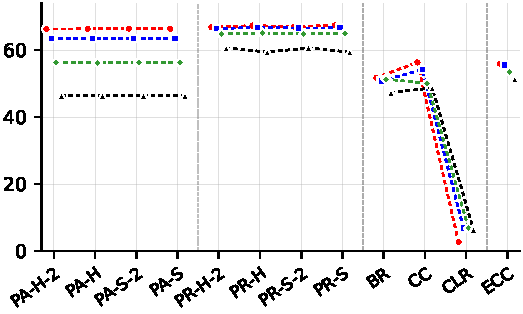
\includegraphics[width=\linewidth]{fig_rf_gpositivepseaac_bv_f1.pdf}\\\scriptsize $f^{1}_{\mathrm{MLC}}$ (\ref{eq:f1mlc}) ($\uparrow$)\end{minipage} & \begin{minipage}{0.32\textwidth}\centering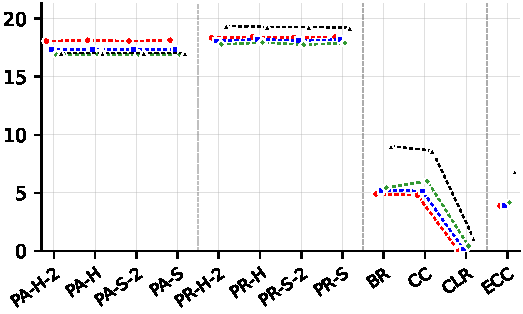
\includegraphics[width=\linewidth]{fig_rf_plantpseaac_bv_f1.pdf}\\\scriptsize $f^{1}_{\mathrm{MLC}}$ (\ref{eq:f1mlc}) ($\uparrow$)\end{minipage} & \begin{minipage}{0.32\textwidth}\centering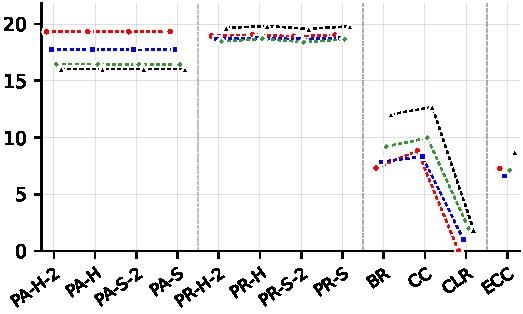
\includegraphics[width=\linewidth]{fig_rf_humanpseaac_bv_f1.pdf}\\\scriptsize $f^{1}_{\mathrm{MLC}}$ (\ref{eq:f1mlc}) ($\uparrow$)\end{minipage} \\[6pt]
\begin{minipage}{0.32\textwidth}\centering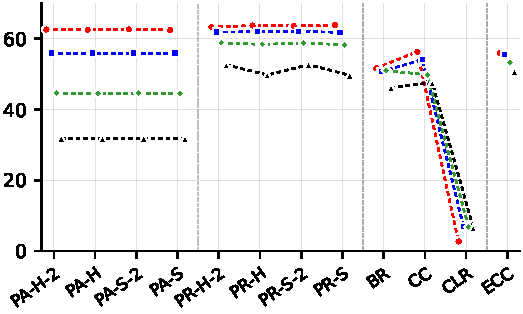
\includegraphics[width=\linewidth]{fig_rf_gpositivepseaac_bv_jaccard.pdf}\\\scriptsize $f^{\mathrm{Jacc}}_{\mathrm{MLC}}$ (\ref{eq:jaccmlc}) ($\uparrow$)\end{minipage} & \begin{minipage}{0.32\textwidth}\centering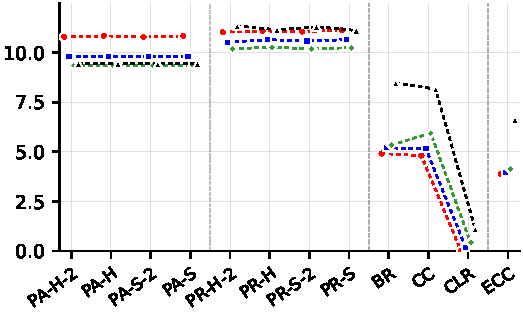
\includegraphics[width=\linewidth]{fig_rf_plantpseaac_bv_jaccard.pdf}\\\scriptsize $f^{\mathrm{Jacc}}_{\mathrm{MLC}}$ (\ref{eq:jaccmlc}) ($\uparrow$)\end{minipage} & \begin{minipage}{0.32\textwidth}\centering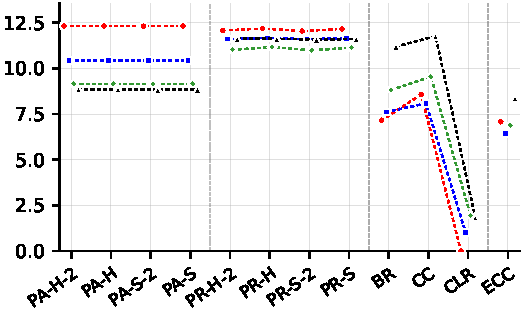
\includegraphics[width=\linewidth]{fig_rf_humanpseaac_bv_jaccard.pdf}\\\scriptsize $f^{\mathrm{Jacc}}_{\mathrm{MLC}}$ (\ref{eq:jaccmlc}) ($\uparrow$)\end{minipage} \\[6pt]
\begin{minipage}{0.32\textwidth}\centering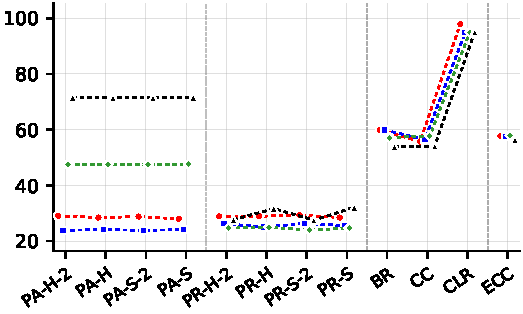
\includegraphics[width=\linewidth]{fig_rf_gpositivepseaac_bv_afrd.pdf}\\\scriptsize AFRD (\ref{eq:afrd}) ($\downarrow$)\end{minipage} & \begin{minipage}{0.32\textwidth}\centering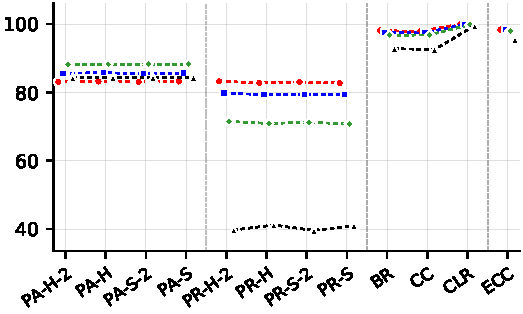
\includegraphics[width=\linewidth]{fig_rf_plantpseaac_bv_afrd.pdf}\\\scriptsize AFRD (\ref{eq:afrd}) ($\downarrow$)\end{minipage} & \begin{minipage}{0.32\textwidth}\centering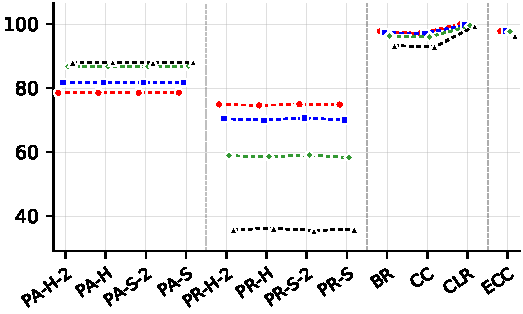
\includegraphics[width=\linewidth]{fig_rf_humanpseaac_bv_afrd.pdf}\\\scriptsize AFRD (\ref{eq:afrd}) ($\downarrow$)\end{minipage} \\[6pt]
\begin{minipage}{0.32\textwidth}\centering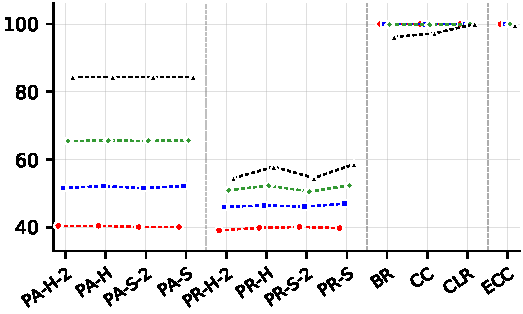
\includegraphics[width=\linewidth]{fig_rf_gpositivepseaac_bv_mfrd.pdf}\\\scriptsize MFRD (\ref{eq:mfrd}) ($\downarrow$)\end{minipage} & \begin{minipage}{0.32\textwidth}\centering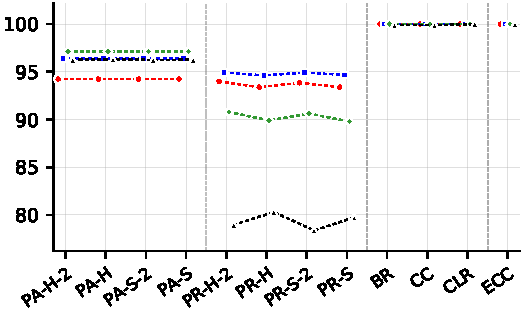
\includegraphics[width=\linewidth]{fig_rf_plantpseaac_bv_mfrd.pdf}\\\scriptsize MFRD (\ref{eq:mfrd}) ($\downarrow$)\end{minipage} & \begin{minipage}{0.32\textwidth}\centering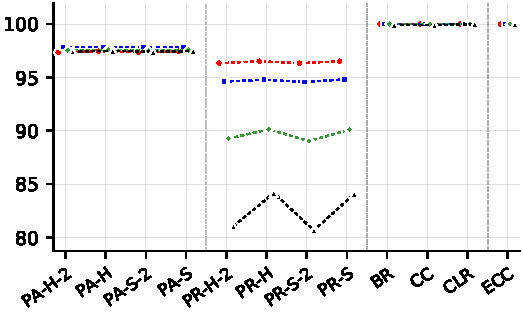
\includegraphics[width=\linewidth]{fig_rf_humanpseaac_bv_mfrd.pdf}\\\scriptsize MFRD (\ref{eq:mfrd}) ($\downarrow$)\end{minipage} \\[6pt]
\end{tabular}
\caption{(Table 4) Average scores (in \%, $y$-axis) over $5\times 5$ cross-validation folds, plotted against the classifiers ($x$-axis): partial-order predictors (PA-H-2, PA-H, PA-S-2, PA-S), preorder predictors (PR-H-2, PR-H, PR-S-2, PR-S), and standard MLC baselines (BR, CC, CLR). Results are color-coded with respect to the noisy level $\alpha$ as follows: \textcolor[HTML]{FF0000}{$\alpha = 0.0$}, \textcolor[HTML]{0000FF}{$\alpha = 0.1$}, \textcolor[HTML]{339933}{$\alpha = 0.2$} and \textcolor[HTML]{000000}{$\alpha = 0.3$}.}
\label{tab:paper_rf_bv_g1}
\end{table}

\FloatBarrier

\subsection{Partial abstention (PartialAbstention)}

\pdfbookmark[3]{(Table 5) Group 1: GpositivePseAAC, PlantPseAAC, HumanPseAAC}{paper-rf-pa-g1}
\begin{table}[!htbp]
\centering
\setlength{\tabcolsep}{2pt}
\renewcommand{\arraystretch}{0.8}
\begin{tabular}{c!{\color{black!25}\vrule width 0.3pt}c!{\color{black!25}\vrule width 0.3pt}c}
\textbf{GpositivePse} & \textbf{plantPse} & \textbf{HumanPse} \\
\begin{minipage}{0.32\textwidth}\centering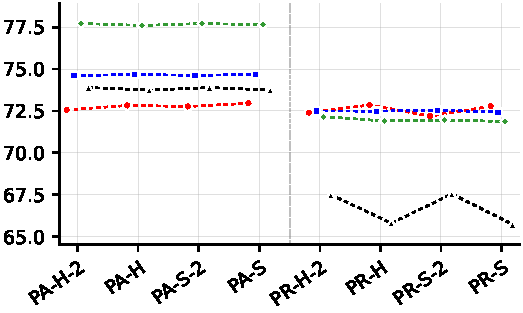
\includegraphics[width=\linewidth]{fig_rf_gpositivepseaac_pa_f1_pa.pdf}\\\scriptsize $f^{1}_{\mathrm{MLC}}$ (\ref{eq:f1mlc}) ($\uparrow$)\end{minipage} & \begin{minipage}{0.32\textwidth}\centering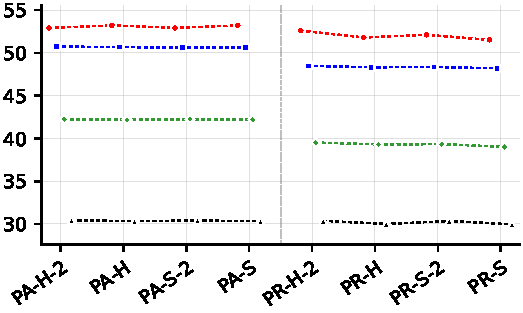
\includegraphics[width=\linewidth]{fig_rf_plantpseaac_pa_f1_pa.pdf}\\\scriptsize $f^{1}_{\mathrm{MLC}}$ (\ref{eq:f1mlc}) ($\uparrow$)\end{minipage} & \begin{minipage}{0.32\textwidth}\centering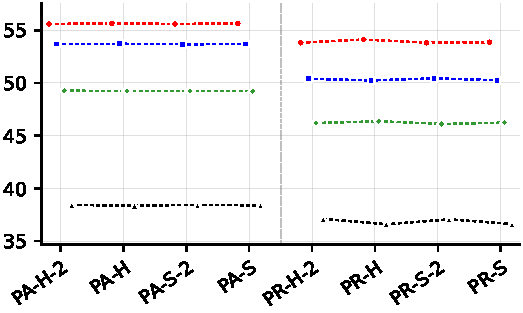
\includegraphics[width=\linewidth]{fig_rf_humanpseaac_pa_f1_pa.pdf}\\\scriptsize $f^{1}_{\mathrm{MLC}}$ (\ref{eq:f1mlc}) ($\uparrow$)\end{minipage} \\[6pt]
\begin{minipage}{0.32\textwidth}\centering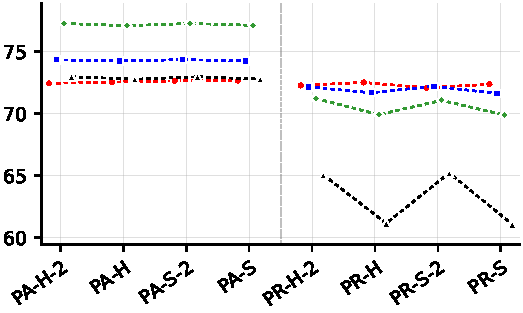
\includegraphics[width=\linewidth]{fig_rf_gpositivepseaac_pa_jaccard_pa.pdf}\\\scriptsize $f^{\mathrm{Jacc}}_{\mathrm{MLC}}$ (\ref{eq:jaccmlc}) ($\uparrow$)\end{minipage} & \begin{minipage}{0.32\textwidth}\centering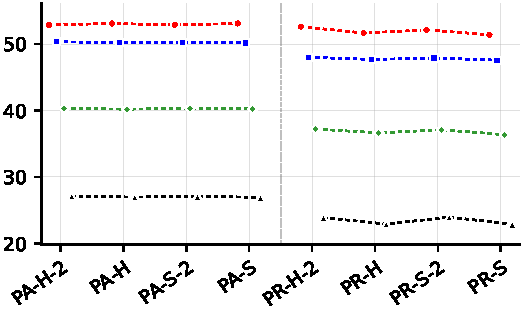
\includegraphics[width=\linewidth]{fig_rf_plantpseaac_pa_jaccard_pa.pdf}\\\scriptsize $f^{\mathrm{Jacc}}_{\mathrm{MLC}}$ (\ref{eq:jaccmlc}) ($\uparrow$)\end{minipage} & \begin{minipage}{0.32\textwidth}\centering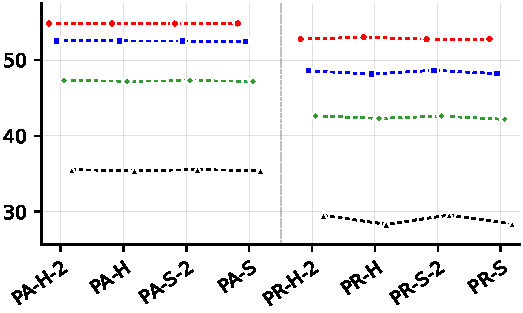
\includegraphics[width=\linewidth]{fig_rf_humanpseaac_pa_jaccard_pa.pdf}\\\scriptsize $f^{\mathrm{Jacc}}_{\mathrm{MLC}}$ (\ref{eq:jaccmlc}) ($\uparrow$)\end{minipage} \\[6pt]
\begin{minipage}{0.32\textwidth}\centering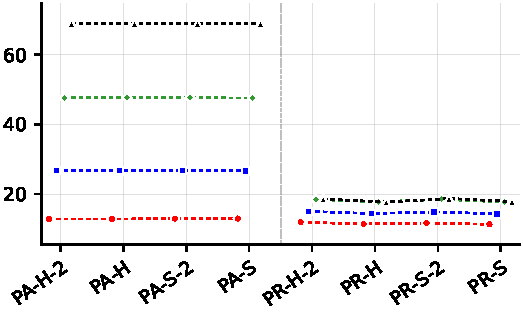
\includegraphics[width=\linewidth]{fig_rf_gpositivepseaac_pa_aabs.pdf}\\\scriptsize $\mathrm{AABS}$ (\ref{eq:aabs}) ($\downarrow$)\end{minipage} & \begin{minipage}{0.32\textwidth}\centering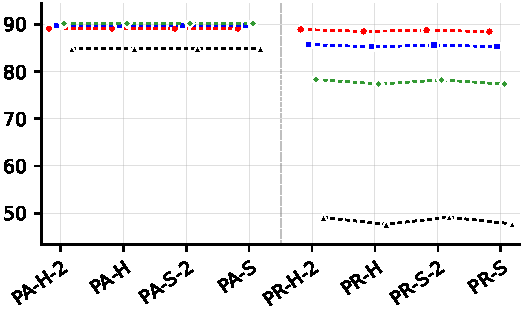
\includegraphics[width=\linewidth]{fig_rf_plantpseaac_pa_aabs.pdf}\\\scriptsize $\mathrm{AABS}$ (\ref{eq:aabs}) ($\downarrow$)\end{minipage} & \begin{minipage}{0.32\textwidth}\centering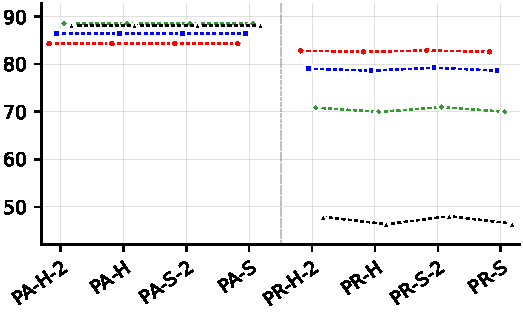
\includegraphics[width=\linewidth]{fig_rf_humanpseaac_pa_aabs.pdf}\\\scriptsize $\mathrm{AABS}$ (\ref{eq:aabs}) ($\downarrow$)\end{minipage} \\[6pt]
\begin{minipage}{0.32\textwidth}\centering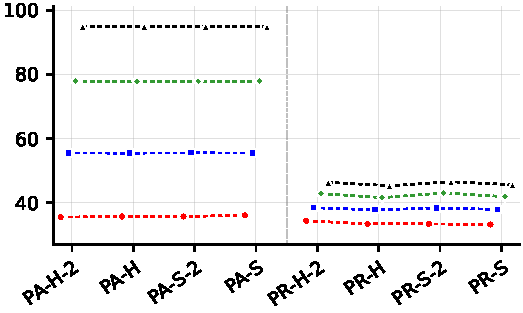
\includegraphics[width=\linewidth]{fig_rf_gpositivepseaac_pa_abs.pdf}\\\scriptsize $\mathrm{ABS}$ (\ref{eq:abs}) ($\downarrow$)\end{minipage} & \begin{minipage}{0.32\textwidth}\centering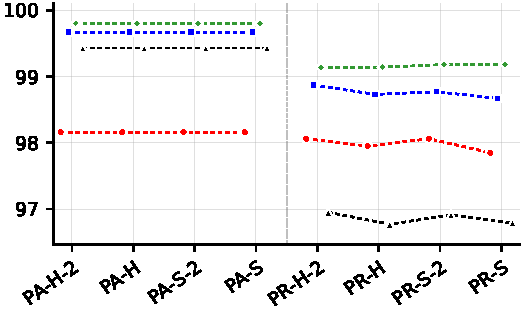
\includegraphics[width=\linewidth]{fig_rf_plantpseaac_pa_abs.pdf}\\\scriptsize $\mathrm{ABS}$ (\ref{eq:abs}) ($\downarrow$)\end{minipage} & \begin{minipage}{0.32\textwidth}\centering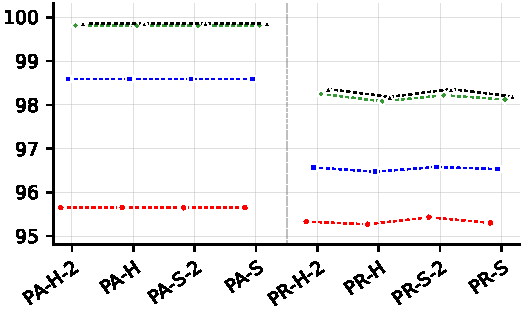
\includegraphics[width=\linewidth]{fig_rf_humanpseaac_pa_abs.pdf}\\\scriptsize $\mathrm{ABS}$ (\ref{eq:abs}) ($\downarrow$)\end{minipage} \\[6pt]
\end{tabular}
\caption{(Table 5) Average scores (in \%, $y$-axis) over $5\times 5$ cross-validation folds, plotted against the classifiers ($x$-axis): partial-order predictors (PA-H-2, PA-H, PA-S-2, PA-S) and preorder predictors (PR-H-2, PR-H, PR-S-2, PR-S). Results are color-coded with respect to the noisy level $\alpha$ as follows: \textcolor[HTML]{FF0000}{$\alpha = 0.0$}, \textcolor[HTML]{0000FF}{$\alpha = 0.1$}, \textcolor[HTML]{339933}{$\alpha = 0.2$} and \textcolor[HTML]{000000}{$\alpha = 0.3$}.}
\label{tab:paper_rf_pa_g1}
\end{table}

\FloatBarrier

\subsection{Experimental results --- appendix tables (RF base learner)}\label{sec:paperapp-rf}

Appendix counterpart of the main Paper results section. Tables All tables share the same 8-metric set (original 5 + 3 revision additions: $f^{\mathrm{Jacc}}_{\mathrm{MLC}}$, macro-$f_1$, micro-$f_1$). G2/G4 = imbalanced datasets, G3/G5 = balanced datasets (split follows the original paper's appendix). G6/G7 = main-paper datasets (GpositivePse, PlantPse, HumanPse) shown with the full metric set; the main body only carries the revised compact Tables 4/5.


\subsubsection{Standard MLC predictions (BinaryVector)}

\pdfbookmark[3]{(Table G2) Group 1: CHD_49, Yeast, enron}{paperapp_g2-rf-bv-g1}
\begin{table}[!htbp]
\centering
\setlength{\tabcolsep}{2pt}
\renewcommand{\arraystretch}{0.65}
\begin{tabular}{c!{\color{black!25}\vrule width 0.3pt}c!{\color{black!25}\vrule width 0.3pt}c}
\textbf{CHD-49} & \textbf{Yeast} & \textbf{enron} \\
\begin{minipage}{0.27\textwidth}\centering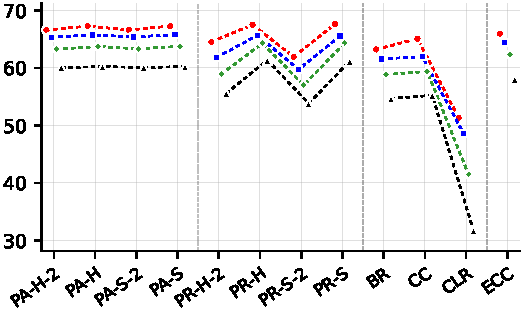
\includegraphics[width=\linewidth]{fig_rf_chd_49_bv_f1.pdf}\\\scriptsize $f^{1}_{\mathrm{MLC}}$ (\ref{eq:f1mlc}) ($\uparrow$)\end{minipage} & \begin{minipage}{0.27\textwidth}\centering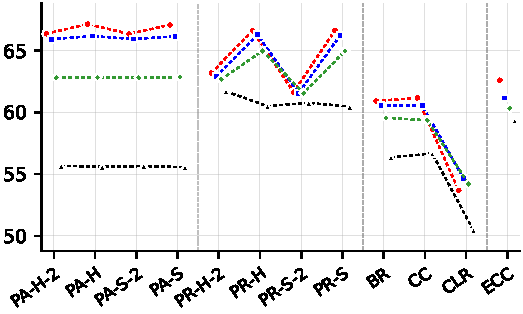
\includegraphics[width=\linewidth]{fig_rf_yeast_bv_f1.pdf}\\\scriptsize $f^{1}_{\mathrm{MLC}}$ (\ref{eq:f1mlc}) ($\uparrow$)\end{minipage} & \begin{minipage}{0.27\textwidth}\centering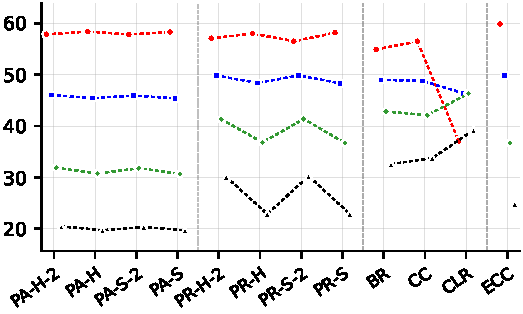
\includegraphics[width=\linewidth]{fig_rf_enron_bv_f1.pdf}\\\scriptsize $f^{1}_{\mathrm{MLC}}$ (\ref{eq:f1mlc}) ($\uparrow$)\end{minipage} \\[8pt]
\begin{minipage}{0.27\textwidth}\centering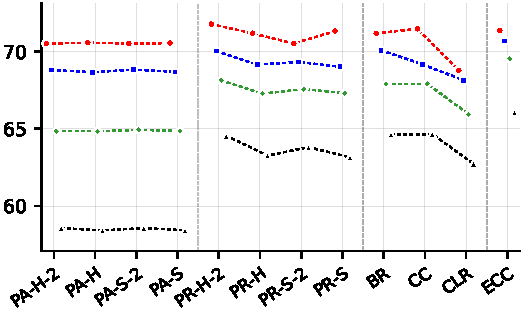
\includegraphics[width=\linewidth]{fig_rf_chd_49_bv_hamming_accuracy.pdf}\\\scriptsize $f^{\mathrm{ham}}_{\mathrm{MLC}}$ (\ref{eq:fham}) ($\uparrow$)\end{minipage} & \begin{minipage}{0.27\textwidth}\centering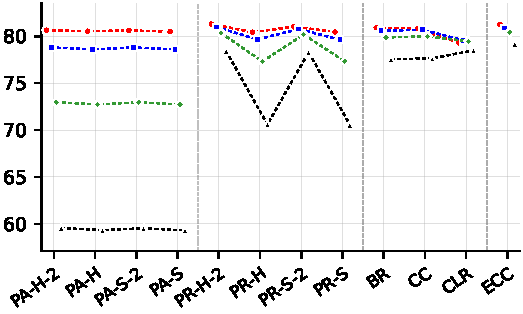
\includegraphics[width=\linewidth]{fig_rf_yeast_bv_hamming_accuracy.pdf}\\\scriptsize $f^{\mathrm{ham}}_{\mathrm{MLC}}$ (\ref{eq:fham}) ($\uparrow$)\end{minipage} & \begin{minipage}{0.27\textwidth}\centering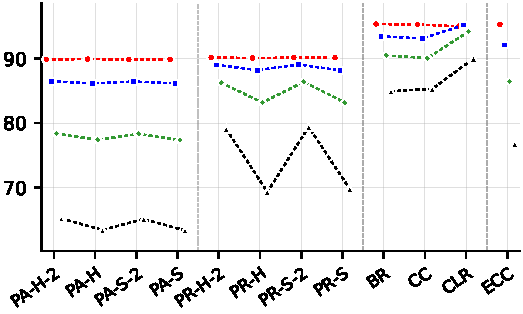
\includegraphics[width=\linewidth]{fig_rf_enron_bv_hamming_accuracy.pdf}\\\scriptsize $f^{\mathrm{ham}}_{\mathrm{MLC}}$ (\ref{eq:fham}) ($\uparrow$)\end{minipage} \\[8pt]
\begin{minipage}{0.27\textwidth}\centering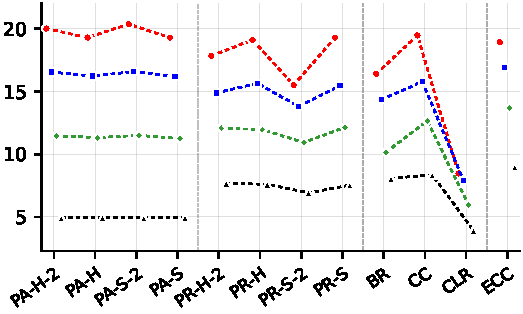
\includegraphics[width=\linewidth]{fig_rf_chd_49_bv_subset0_1.pdf}\\\scriptsize $f^{\mathrm{sub}}_{\mathrm{MLC}}$ (\ref{eq:fsub}) ($\uparrow$)\end{minipage} & \begin{minipage}{0.27\textwidth}\centering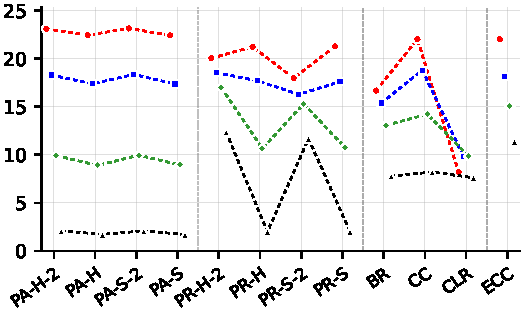
\includegraphics[width=\linewidth]{fig_rf_yeast_bv_subset0_1.pdf}\\\scriptsize $f^{\mathrm{sub}}_{\mathrm{MLC}}$ (\ref{eq:fsub}) ($\uparrow$)\end{minipage} & \begin{minipage}{0.27\textwidth}\centering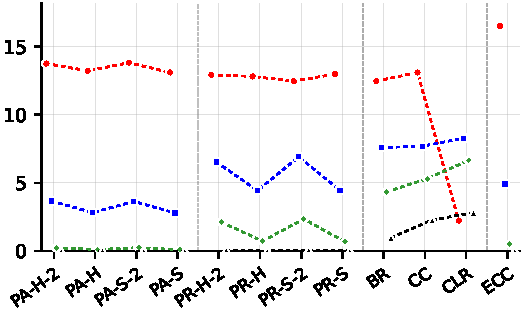
\includegraphics[width=\linewidth]{fig_rf_enron_bv_subset0_1.pdf}\\\scriptsize $f^{\mathrm{sub}}_{\mathrm{MLC}}$ (\ref{eq:fsub}) ($\uparrow$)\end{minipage} \\[8pt]
\begin{minipage}{0.27\textwidth}\centering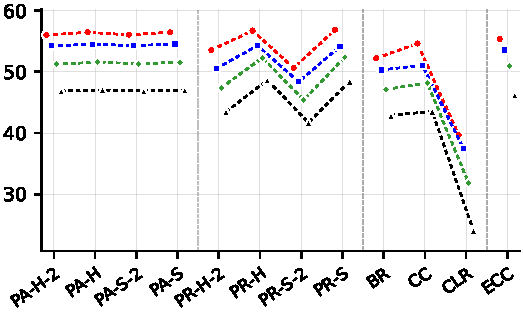
\includegraphics[width=\linewidth]{fig_rf_chd_49_bv_jaccard.pdf}\\\scriptsize $f^{\mathrm{Jacc}}_{\mathrm{MLC}}$ (\ref{eq:jaccmlc}) ($\uparrow$)\end{minipage} & \begin{minipage}{0.27\textwidth}\centering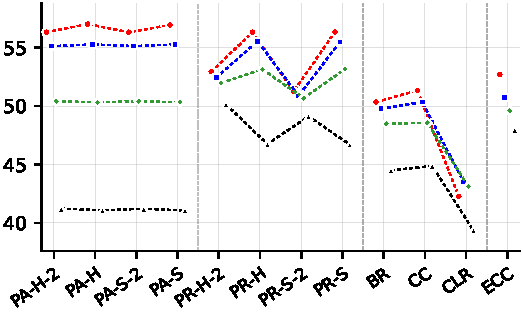
\includegraphics[width=\linewidth]{fig_rf_yeast_bv_jaccard.pdf}\\\scriptsize $f^{\mathrm{Jacc}}_{\mathrm{MLC}}$ (\ref{eq:jaccmlc}) ($\uparrow$)\end{minipage} & \begin{minipage}{0.27\textwidth}\centering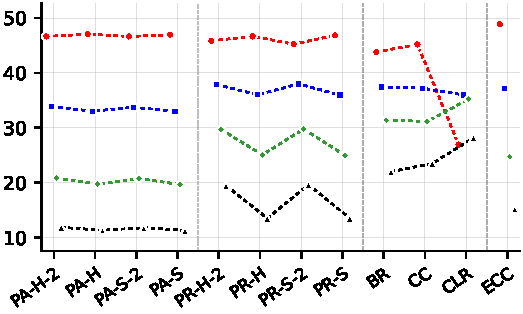
\includegraphics[width=\linewidth]{fig_rf_enron_bv_jaccard.pdf}\\\scriptsize $f^{\mathrm{Jacc}}_{\mathrm{MLC}}$ (\ref{eq:jaccmlc}) ($\uparrow$)\end{minipage} \\[8pt]
\begin{minipage}{0.27\textwidth}\centering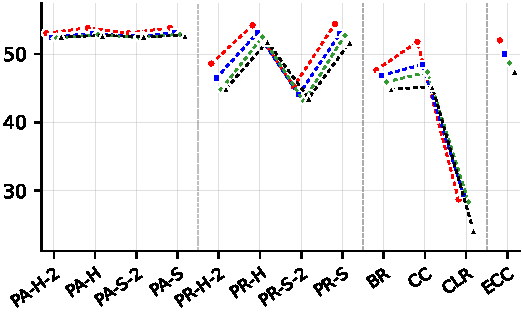
\includegraphics[width=\linewidth]{fig_rf_chd_49_bv_macro_f1.pdf}\\\scriptsize macro-$f_1$ (\ref{eq:macrof1}) ($\uparrow$)\end{minipage} & \begin{minipage}{0.27\textwidth}\centering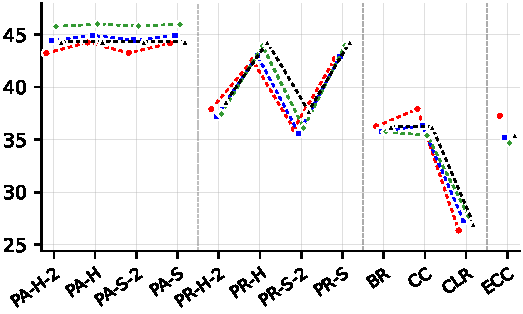
\includegraphics[width=\linewidth]{fig_rf_yeast_bv_macro_f1.pdf}\\\scriptsize macro-$f_1$ (\ref{eq:macrof1}) ($\uparrow$)\end{minipage} & \begin{minipage}{0.27\textwidth}\centering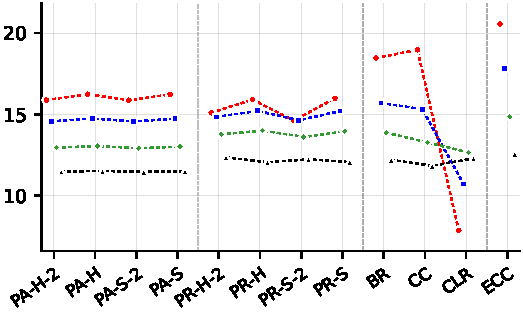
\includegraphics[width=\linewidth]{fig_rf_enron_bv_macro_f1.pdf}\\\scriptsize macro-$f_1$ (\ref{eq:macrof1}) ($\uparrow$)\end{minipage} \\[8pt]
\begin{minipage}{0.27\textwidth}\centering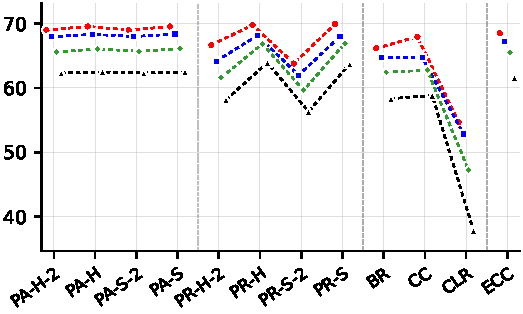
\includegraphics[width=\linewidth]{fig_rf_chd_49_bv_micro_f1.pdf}\\\scriptsize micro-$f_1$ (\ref{eq:microf1}) ($\uparrow$)\end{minipage} & \begin{minipage}{0.27\textwidth}\centering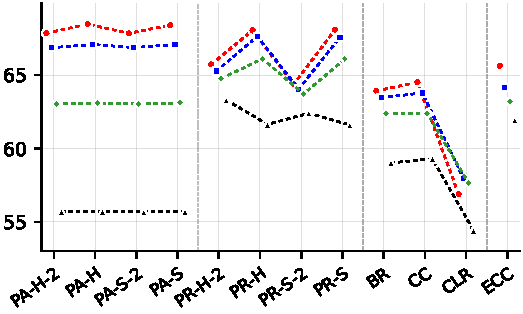
\includegraphics[width=\linewidth]{fig_rf_yeast_bv_micro_f1.pdf}\\\scriptsize micro-$f_1$ (\ref{eq:microf1}) ($\uparrow$)\end{minipage} & \begin{minipage}{0.27\textwidth}\centering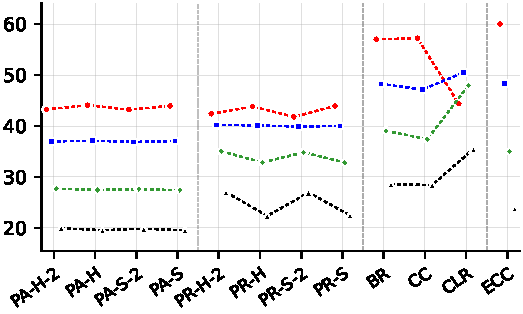
\includegraphics[width=\linewidth]{fig_rf_enron_bv_micro_f1.pdf}\\\scriptsize micro-$f_1$ (\ref{eq:microf1}) ($\uparrow$)\end{minipage} \\[8pt]
\begin{minipage}{0.27\textwidth}\centering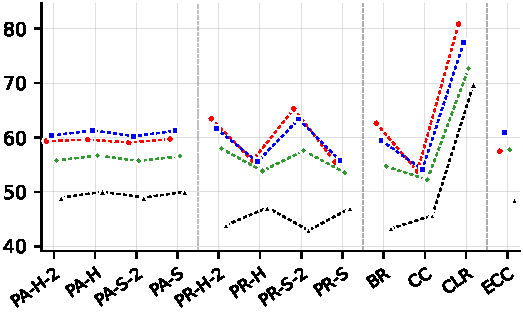
\includegraphics[width=\linewidth]{fig_rf_chd_49_bv_afrd.pdf}\\\scriptsize AFRD (\ref{eq:afrd}) ($\downarrow$)\end{minipage} & \begin{minipage}{0.27\textwidth}\centering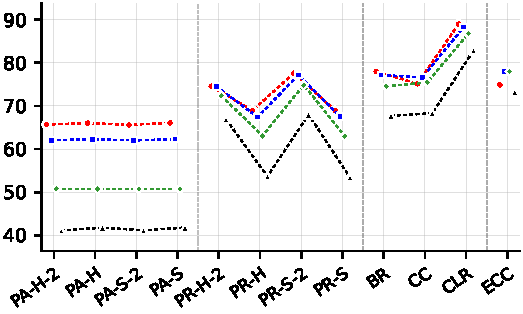
\includegraphics[width=\linewidth]{fig_rf_yeast_bv_afrd.pdf}\\\scriptsize AFRD (\ref{eq:afrd}) ($\downarrow$)\end{minipage} & \begin{minipage}{0.27\textwidth}\centering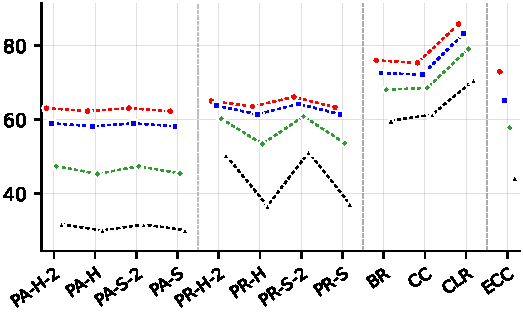
\includegraphics[width=\linewidth]{fig_rf_enron_bv_afrd.pdf}\\\scriptsize AFRD (\ref{eq:afrd}) ($\downarrow$)\end{minipage} \\[8pt]
\begin{minipage}{0.27\textwidth}\centering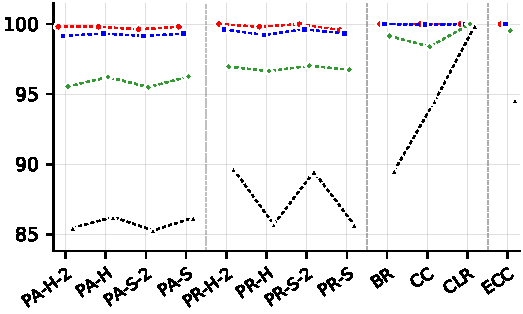
\includegraphics[width=\linewidth]{fig_rf_chd_49_bv_mfrd.pdf}\\\scriptsize MFRD (\ref{eq:mfrd}) ($\downarrow$)\end{minipage} & \begin{minipage}{0.27\textwidth}\centering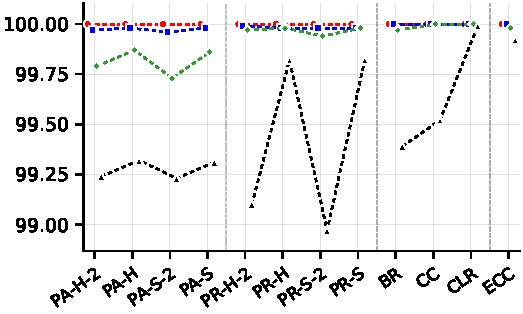
\includegraphics[width=\linewidth]{fig_rf_yeast_bv_mfrd.pdf}\\\scriptsize MFRD (\ref{eq:mfrd}) ($\downarrow$)\end{minipage} & \begin{minipage}{0.27\textwidth}\centering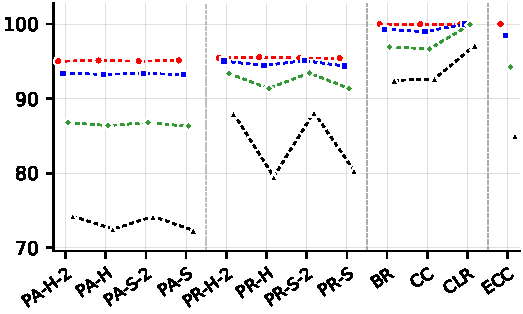
\includegraphics[width=\linewidth]{fig_rf_enron_bv_mfrd.pdf}\\\scriptsize MFRD (\ref{eq:mfrd}) ($\downarrow$)\end{minipage} \\[8pt]
\end{tabular}
\caption{(Table G2) Average scores (in \%, $y$-axis) over $5\times 5$ cross-validation folds, plotted against the classifiers ($x$-axis): partial-order predictors (PA-H-2, PA-H, PA-S-2, PA-S), preorder predictors (PR-H-2, PR-H, PR-S-2, PR-S), and standard MLC baselines (BR, CC, CLR). Results are color-coded with respect to the noisy level $\alpha$ as follows: \textcolor[HTML]{FF0000}{$\alpha = 0.0$}, \textcolor[HTML]{0000FF}{$\alpha = 0.1$}, \textcolor[HTML]{339933}{$\alpha = 0.2$} and \textcolor[HTML]{000000}{$\alpha = 0.3$}.}
\label{tab:paperapp_g2_rf_bv_g1}
\end{table}

\FloatBarrier

\pdfbookmark[3]{(Table G3) Group 1: emotions, scene, Water-quality}{paperapp_g3-rf-bv-g1}
\begin{table}[!htbp]
\centering
\setlength{\tabcolsep}{2pt}
\renewcommand{\arraystretch}{0.65}
\begin{tabular}{c!{\color{black!25}\vrule width 0.3pt}c!{\color{black!25}\vrule width 0.3pt}c}
\textbf{emotions} & \textbf{scene} & \textbf{Water-quality} \\
\begin{minipage}{0.27\textwidth}\centering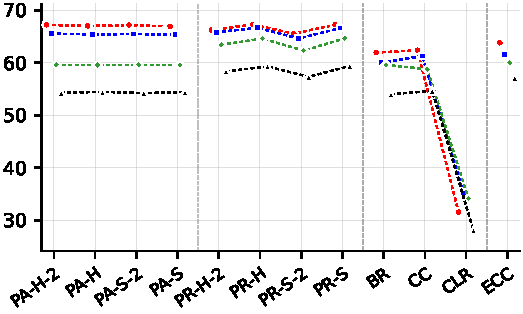
\includegraphics[width=\linewidth]{fig_rf_emotions_bv_f1.pdf}\\\scriptsize $f^{1}_{\mathrm{MLC}}$ (\ref{eq:f1mlc}) ($\uparrow$)\end{minipage} & \begin{minipage}{0.27\textwidth}\centering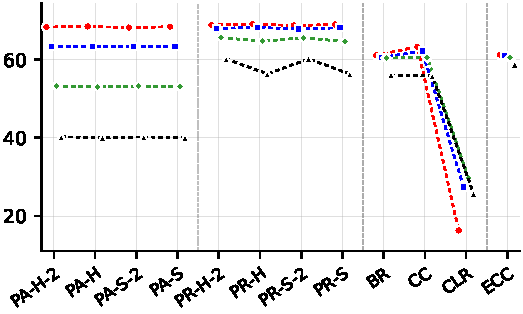
\includegraphics[width=\linewidth]{fig_rf_scene_bv_f1.pdf}\\\scriptsize $f^{1}_{\mathrm{MLC}}$ (\ref{eq:f1mlc}) ($\uparrow$)\end{minipage} & \begin{minipage}{0.27\textwidth}\centering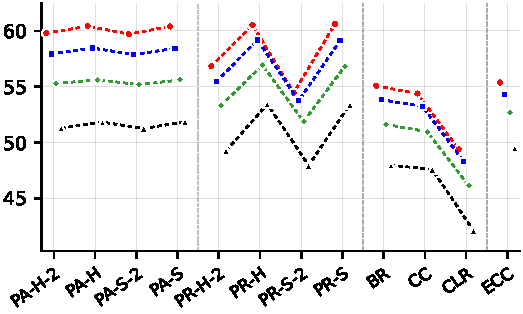
\includegraphics[width=\linewidth]{fig_rf_waterquality_bv_f1.pdf}\\\scriptsize $f^{1}_{\mathrm{MLC}}$ (\ref{eq:f1mlc}) ($\uparrow$)\end{minipage} \\[8pt]
\begin{minipage}{0.27\textwidth}\centering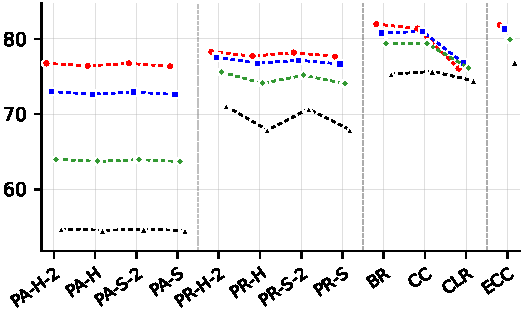
\includegraphics[width=\linewidth]{fig_rf_emotions_bv_hamming_accuracy.pdf}\\\scriptsize $f^{\mathrm{ham}}_{\mathrm{MLC}}$ (\ref{eq:fham}) ($\uparrow$)\end{minipage} & \begin{minipage}{0.27\textwidth}\centering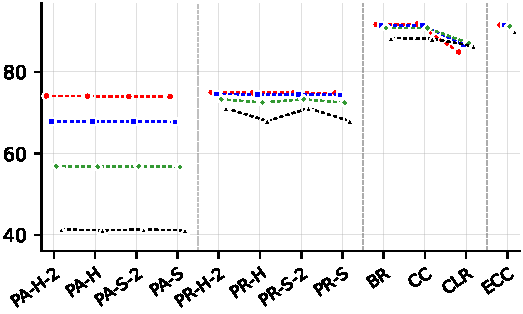
\includegraphics[width=\linewidth]{fig_rf_scene_bv_hamming_accuracy.pdf}\\\scriptsize $f^{\mathrm{ham}}_{\mathrm{MLC}}$ (\ref{eq:fham}) ($\uparrow$)\end{minipage} & \begin{minipage}{0.27\textwidth}\centering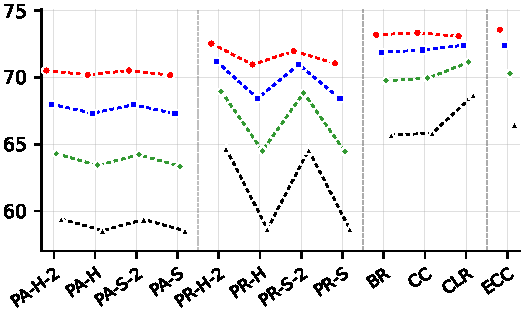
\includegraphics[width=\linewidth]{fig_rf_waterquality_bv_hamming_accuracy.pdf}\\\scriptsize $f^{\mathrm{ham}}_{\mathrm{MLC}}$ (\ref{eq:fham}) ($\uparrow$)\end{minipage} \\[8pt]
\begin{minipage}{0.27\textwidth}\centering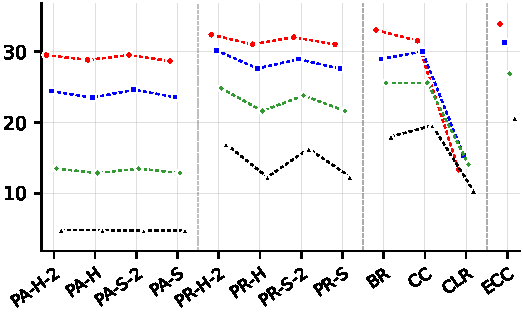
\includegraphics[width=\linewidth]{fig_rf_emotions_bv_subset0_1.pdf}\\\scriptsize $f^{\mathrm{sub}}_{\mathrm{MLC}}$ (\ref{eq:fsub}) ($\uparrow$)\end{minipage} & \begin{minipage}{0.27\textwidth}\centering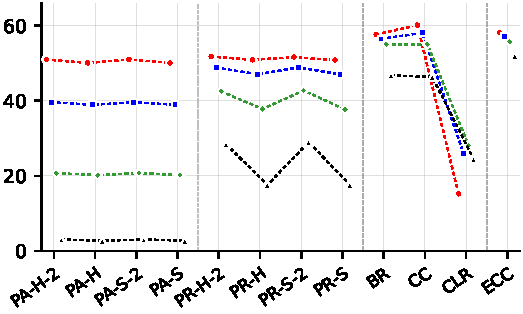
\includegraphics[width=\linewidth]{fig_rf_scene_bv_subset0_1.pdf}\\\scriptsize $f^{\mathrm{sub}}_{\mathrm{MLC}}$ (\ref{eq:fsub}) ($\uparrow$)\end{minipage} & \begin{minipage}{0.27\textwidth}\centering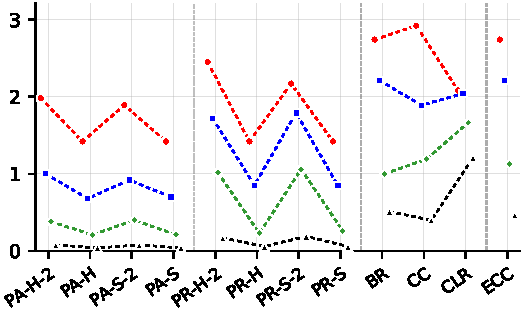
\includegraphics[width=\linewidth]{fig_rf_waterquality_bv_subset0_1.pdf}\\\scriptsize $f^{\mathrm{sub}}_{\mathrm{MLC}}$ (\ref{eq:fsub}) ($\uparrow$)\end{minipage} \\[8pt]
\begin{minipage}{0.27\textwidth}\centering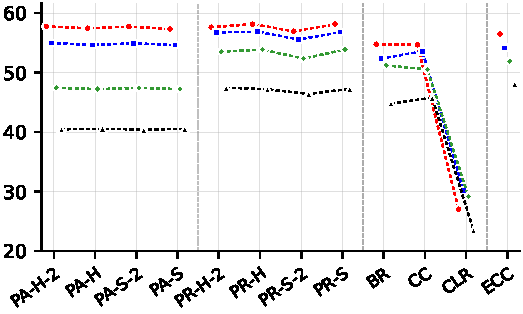
\includegraphics[width=\linewidth]{fig_rf_emotions_bv_jaccard.pdf}\\\scriptsize $f^{\mathrm{Jacc}}_{\mathrm{MLC}}$ (\ref{eq:jaccmlc}) ($\uparrow$)\end{minipage} & \begin{minipage}{0.27\textwidth}\centering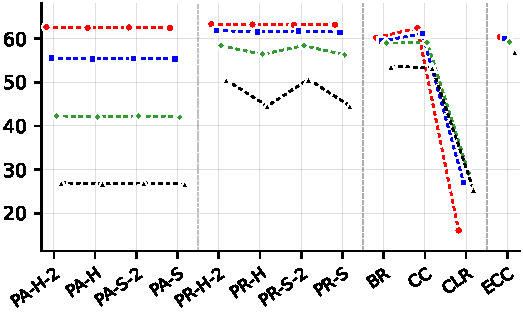
\includegraphics[width=\linewidth]{fig_rf_scene_bv_jaccard.pdf}\\\scriptsize $f^{\mathrm{Jacc}}_{\mathrm{MLC}}$ (\ref{eq:jaccmlc}) ($\uparrow$)\end{minipage} & \begin{minipage}{0.27\textwidth}\centering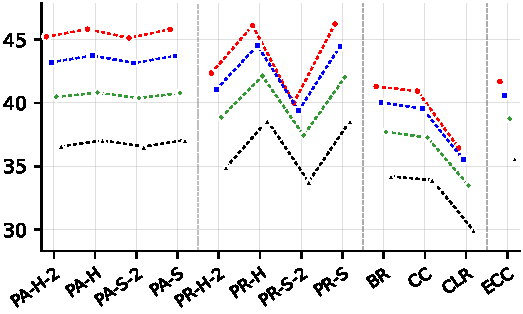
\includegraphics[width=\linewidth]{fig_rf_waterquality_bv_jaccard.pdf}\\\scriptsize $f^{\mathrm{Jacc}}_{\mathrm{MLC}}$ (\ref{eq:jaccmlc}) ($\uparrow$)\end{minipage} \\[8pt]
\begin{minipage}{0.27\textwidth}\centering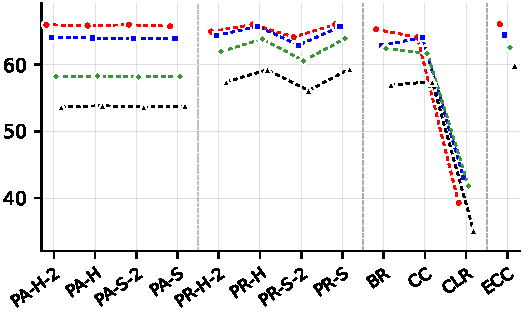
\includegraphics[width=\linewidth]{fig_rf_emotions_bv_macro_f1.pdf}\\\scriptsize macro-$f_1$ (\ref{eq:macrof1}) ($\uparrow$)\end{minipage} & \begin{minipage}{0.27\textwidth}\centering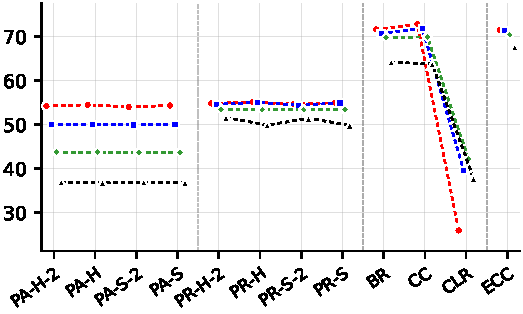
\includegraphics[width=\linewidth]{fig_rf_scene_bv_macro_f1.pdf}\\\scriptsize macro-$f_1$ (\ref{eq:macrof1}) ($\uparrow$)\end{minipage} & \begin{minipage}{0.27\textwidth}\centering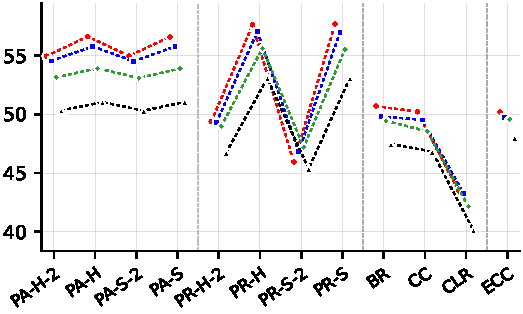
\includegraphics[width=\linewidth]{fig_rf_waterquality_bv_macro_f1.pdf}\\\scriptsize macro-$f_1$ (\ref{eq:macrof1}) ($\uparrow$)\end{minipage} \\[8pt]
\begin{minipage}{0.27\textwidth}\centering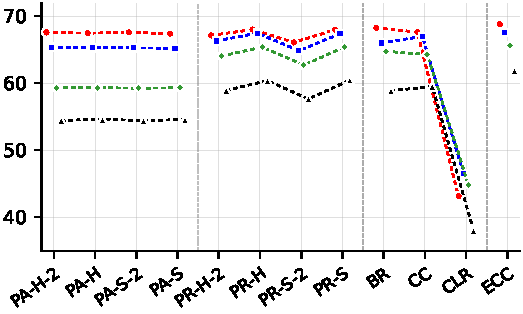
\includegraphics[width=\linewidth]{fig_rf_emotions_bv_micro_f1.pdf}\\\scriptsize micro-$f_1$ (\ref{eq:microf1}) ($\uparrow$)\end{minipage} & \begin{minipage}{0.27\textwidth}\centering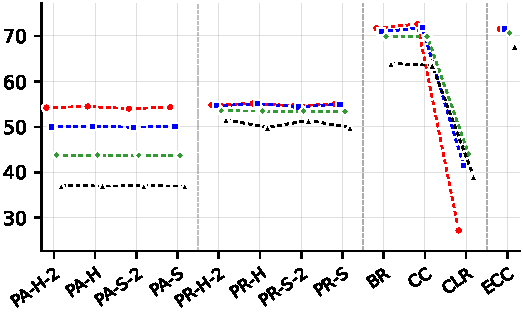
\includegraphics[width=\linewidth]{fig_rf_scene_bv_micro_f1.pdf}\\\scriptsize micro-$f_1$ (\ref{eq:microf1}) ($\uparrow$)\end{minipage} & \begin{minipage}{0.27\textwidth}\centering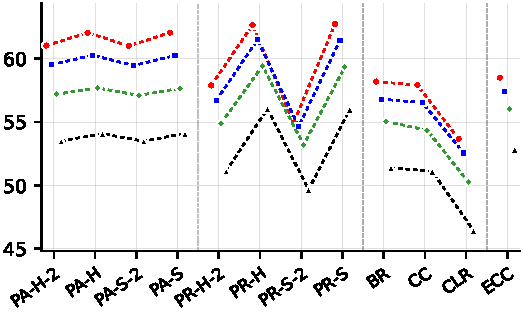
\includegraphics[width=\linewidth]{fig_rf_waterquality_bv_micro_f1.pdf}\\\scriptsize micro-$f_1$ (\ref{eq:microf1}) ($\uparrow$)\end{minipage} \\[8pt]
\begin{minipage}{0.27\textwidth}\centering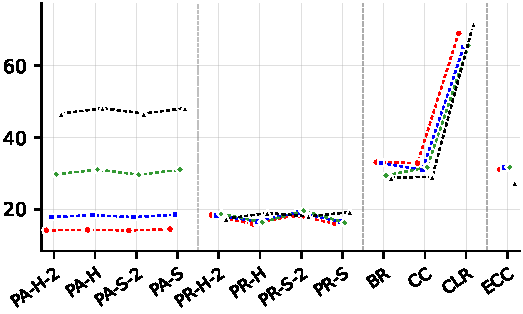
\includegraphics[width=\linewidth]{fig_rf_emotions_bv_afrd.pdf}\\\scriptsize AFRD (\ref{eq:afrd}) ($\downarrow$)\end{minipage} & \begin{minipage}{0.27\textwidth}\centering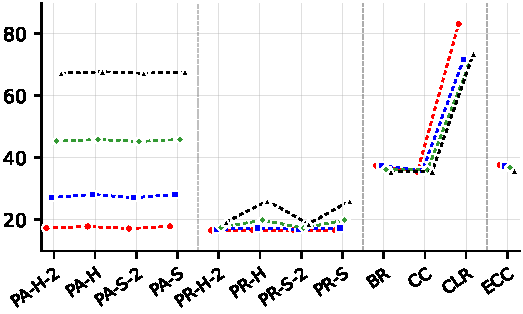
\includegraphics[width=\linewidth]{fig_rf_scene_bv_afrd.pdf}\\\scriptsize AFRD (\ref{eq:afrd}) ($\downarrow$)\end{minipage} & \begin{minipage}{0.27\textwidth}\centering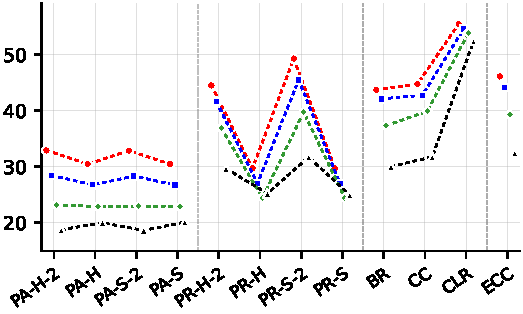
\includegraphics[width=\linewidth]{fig_rf_waterquality_bv_afrd.pdf}\\\scriptsize AFRD (\ref{eq:afrd}) ($\downarrow$)\end{minipage} \\[8pt]
\begin{minipage}{0.27\textwidth}\centering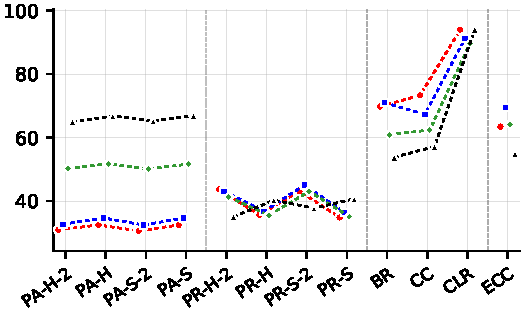
\includegraphics[width=\linewidth]{fig_rf_emotions_bv_mfrd.pdf}\\\scriptsize MFRD (\ref{eq:mfrd}) ($\downarrow$)\end{minipage} & \begin{minipage}{0.27\textwidth}\centering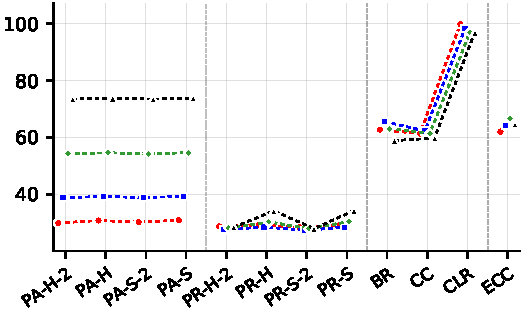
\includegraphics[width=\linewidth]{fig_rf_scene_bv_mfrd.pdf}\\\scriptsize MFRD (\ref{eq:mfrd}) ($\downarrow$)\end{minipage} & \begin{minipage}{0.27\textwidth}\centering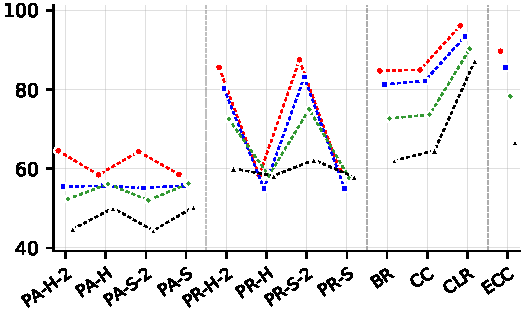
\includegraphics[width=\linewidth]{fig_rf_waterquality_bv_mfrd.pdf}\\\scriptsize MFRD (\ref{eq:mfrd}) ($\downarrow$)\end{minipage} \\[8pt]
\end{tabular}
\caption{(Table G3) Average scores (in \%, $y$-axis) over $5\times 5$ cross-validation folds, plotted against the classifiers ($x$-axis): partial-order predictors (PA-H-2, PA-H, PA-S-2, PA-S), preorder predictors (PR-H-2, PR-H, PR-S-2, PR-S), and standard MLC baselines (BR, CC, CLR). Results are color-coded with respect to the noisy level $\alpha$ as follows: \textcolor[HTML]{FF0000}{$\alpha = 0.0$}, \textcolor[HTML]{0000FF}{$\alpha = 0.1$}, \textcolor[HTML]{339933}{$\alpha = 0.2$} and \textcolor[HTML]{000000}{$\alpha = 0.3$}.}
\label{tab:paperapp_g3_rf_bv_g1}
\end{table}

\FloatBarrier

\subsubsection{Partial abstention (PartialAbstention)}

\pdfbookmark[3]{(Table G4) Group 1: CHD_49, Yeast, enron}{paperapp_g4-rf-pa-g1}
\begin{table}[!htbp]
\centering
\setlength{\tabcolsep}{2pt}
\renewcommand{\arraystretch}{0.65}
\begin{tabular}{c!{\color{black!25}\vrule width 0.3pt}c!{\color{black!25}\vrule width 0.3pt}c}
\textbf{CHD-49} & \textbf{Yeast} & \textbf{enron} \\
\begin{minipage}{0.27\textwidth}\centering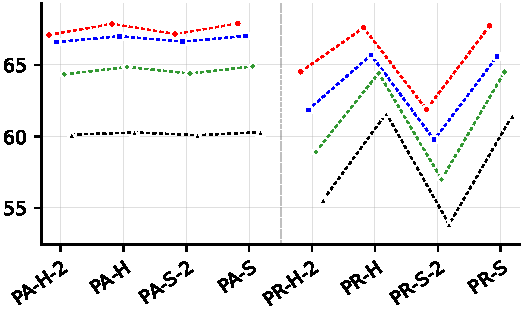
\includegraphics[width=\linewidth]{fig_rf_chd_49_pa_f1_pa.pdf}\\\scriptsize $f^{1}_{\mathrm{MLC}}$ (\ref{eq:f1mlc}) ($\uparrow$)\end{minipage} & \begin{minipage}{0.27\textwidth}\centering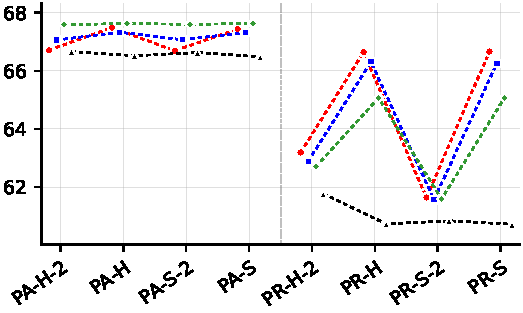
\includegraphics[width=\linewidth]{fig_rf_yeast_pa_f1_pa.pdf}\\\scriptsize $f^{1}_{\mathrm{MLC}}$ (\ref{eq:f1mlc}) ($\uparrow$)\end{minipage} & \begin{minipage}{0.27\textwidth}\centering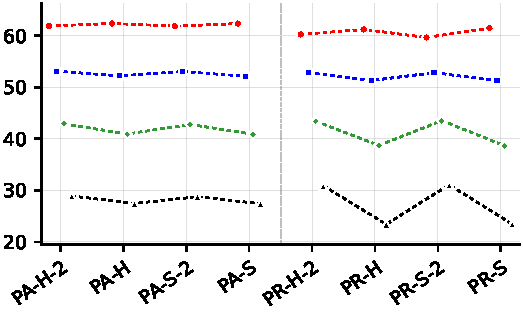
\includegraphics[width=\linewidth]{fig_rf_enron_pa_f1_pa.pdf}\\\scriptsize $f^{1}_{\mathrm{MLC}}$ (\ref{eq:f1mlc}) ($\uparrow$)\end{minipage} \\[8pt]
\begin{minipage}{0.27\textwidth}\centering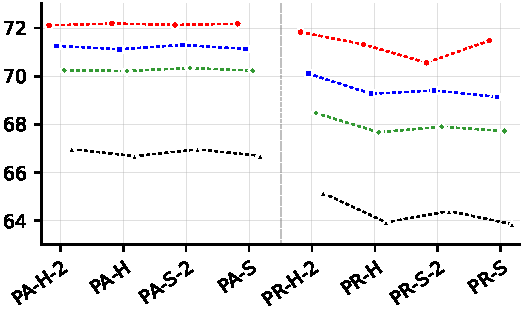
\includegraphics[width=\linewidth]{fig_rf_chd_49_pa_hamming_accuracy_pa.pdf}\\\scriptsize $f^{\mathrm{ham}}_{\mathrm{MLC}}$ (\ref{eq:fham}) ($\uparrow$)\end{minipage} & \begin{minipage}{0.27\textwidth}\centering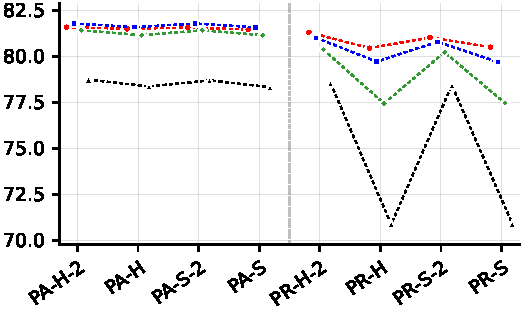
\includegraphics[width=\linewidth]{fig_rf_yeast_pa_hamming_accuracy_pa.pdf}\\\scriptsize $f^{\mathrm{ham}}_{\mathrm{MLC}}$ (\ref{eq:fham}) ($\uparrow$)\end{minipage} & \begin{minipage}{0.27\textwidth}\centering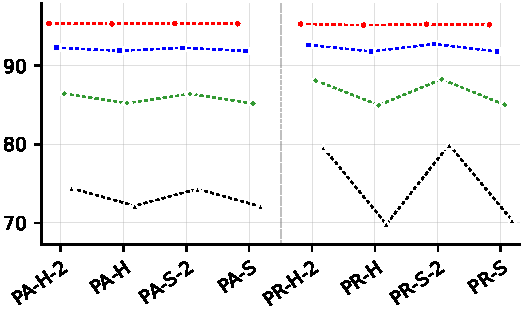
\includegraphics[width=\linewidth]{fig_rf_enron_pa_hamming_accuracy_pa.pdf}\\\scriptsize $f^{\mathrm{ham}}_{\mathrm{MLC}}$ (\ref{eq:fham}) ($\uparrow$)\end{minipage} \\[8pt]
\begin{minipage}{0.27\textwidth}\centering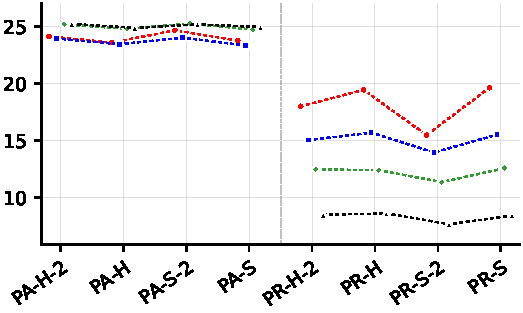
\includegraphics[width=\linewidth]{fig_rf_chd_49_pa_subset0_1_pa.pdf}\\\scriptsize $f^{\mathrm{sub}}_{\mathrm{MLC}}$ (\ref{eq:fsub}) ($\uparrow$)\end{minipage} & \begin{minipage}{0.27\textwidth}\centering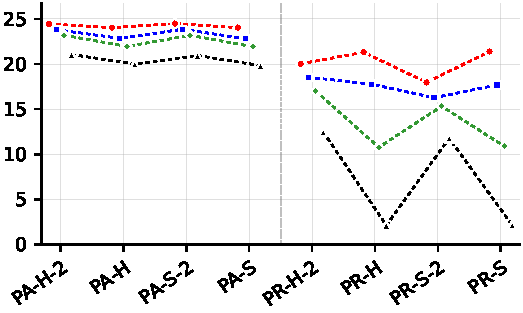
\includegraphics[width=\linewidth]{fig_rf_yeast_pa_subset0_1_pa.pdf}\\\scriptsize $f^{\mathrm{sub}}_{\mathrm{MLC}}$ (\ref{eq:fsub}) ($\uparrow$)\end{minipage} & \begin{minipage}{0.27\textwidth}\centering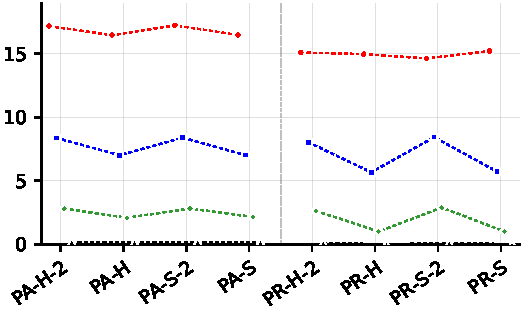
\includegraphics[width=\linewidth]{fig_rf_enron_pa_subset0_1_pa.pdf}\\\scriptsize $f^{\mathrm{sub}}_{\mathrm{MLC}}$ (\ref{eq:fsub}) ($\uparrow$)\end{minipage} \\[8pt]
\begin{minipage}{0.27\textwidth}\centering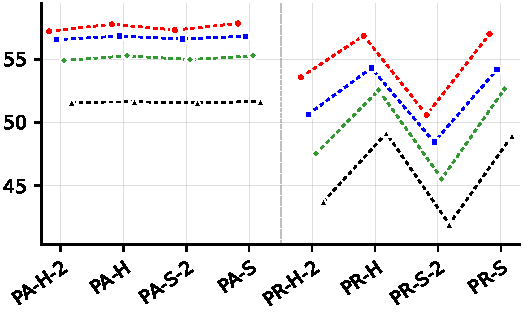
\includegraphics[width=\linewidth]{fig_rf_chd_49_pa_jaccard_pa.pdf}\\\scriptsize $f^{\mathrm{Jacc}}_{\mathrm{MLC}}$ (\ref{eq:jaccmlc}) ($\uparrow$)\end{minipage} & \begin{minipage}{0.27\textwidth}\centering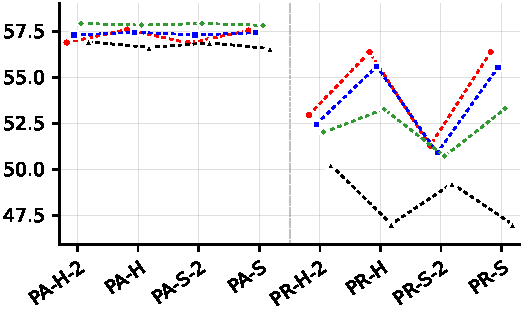
\includegraphics[width=\linewidth]{fig_rf_yeast_pa_jaccard_pa.pdf}\\\scriptsize $f^{\mathrm{Jacc}}_{\mathrm{MLC}}$ (\ref{eq:jaccmlc}) ($\uparrow$)\end{minipage} & \begin{minipage}{0.27\textwidth}\centering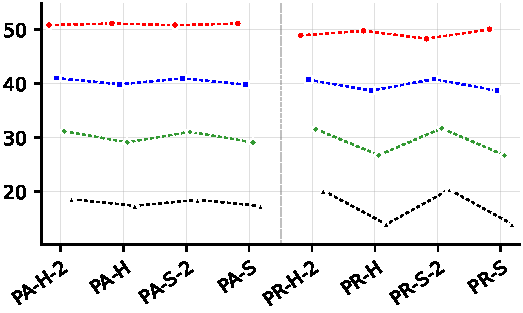
\includegraphics[width=\linewidth]{fig_rf_enron_pa_jaccard_pa.pdf}\\\scriptsize $f^{\mathrm{Jacc}}_{\mathrm{MLC}}$ (\ref{eq:jaccmlc}) ($\uparrow$)\end{minipage} \\[8pt]
\begin{minipage}{0.27\textwidth}\centering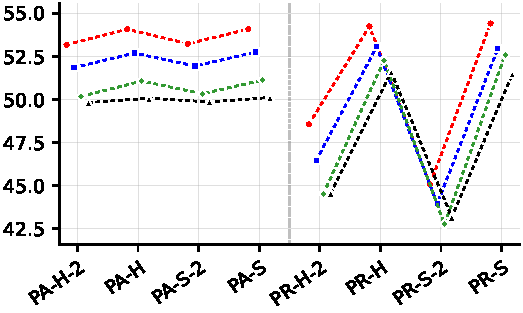
\includegraphics[width=\linewidth]{fig_rf_chd_49_pa_macro_f1_pa.pdf}\\\scriptsize macro-$f_1$ (\ref{eq:macrof1}) ($\uparrow$)\end{minipage} & \begin{minipage}{0.27\textwidth}\centering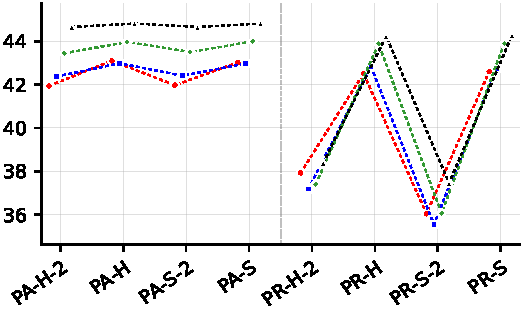
\includegraphics[width=\linewidth]{fig_rf_yeast_pa_macro_f1_pa.pdf}\\\scriptsize macro-$f_1$ (\ref{eq:macrof1}) ($\uparrow$)\end{minipage} & \begin{minipage}{0.27\textwidth}\centering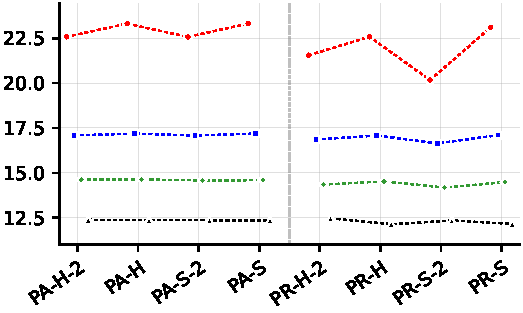
\includegraphics[width=\linewidth]{fig_rf_enron_pa_macro_f1_pa.pdf}\\\scriptsize macro-$f_1$ (\ref{eq:macrof1}) ($\uparrow$)\end{minipage} \\[8pt]
\begin{minipage}{0.27\textwidth}\centering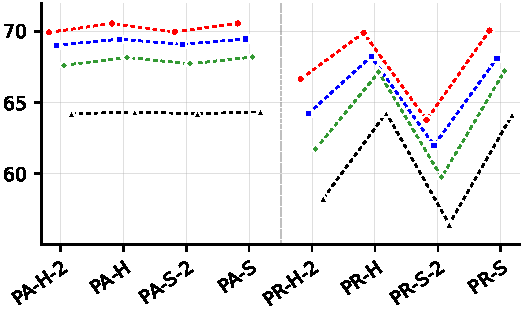
\includegraphics[width=\linewidth]{fig_rf_chd_49_pa_micro_f1_pa.pdf}\\\scriptsize micro-$f_1$ (\ref{eq:microf1}) ($\uparrow$)\end{minipage} & \begin{minipage}{0.27\textwidth}\centering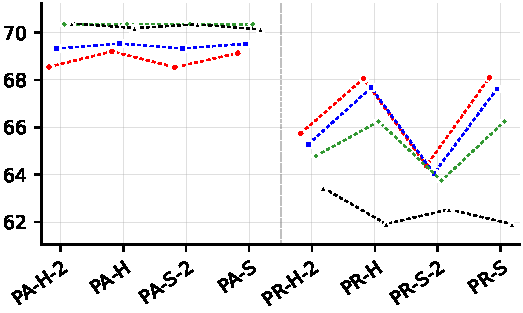
\includegraphics[width=\linewidth]{fig_rf_yeast_pa_micro_f1_pa.pdf}\\\scriptsize micro-$f_1$ (\ref{eq:microf1}) ($\uparrow$)\end{minipage} & \begin{minipage}{0.27\textwidth}\centering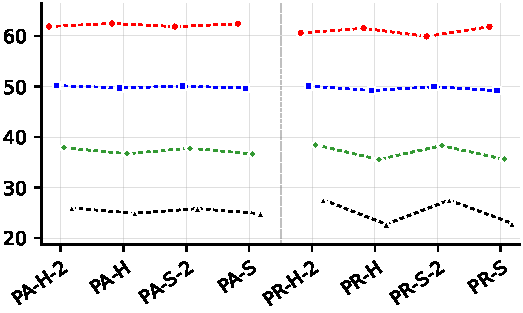
\includegraphics[width=\linewidth]{fig_rf_enron_pa_micro_f1_pa.pdf}\\\scriptsize micro-$f_1$ (\ref{eq:microf1}) ($\uparrow$)\end{minipage} \\[8pt]
\begin{minipage}{0.27\textwidth}\centering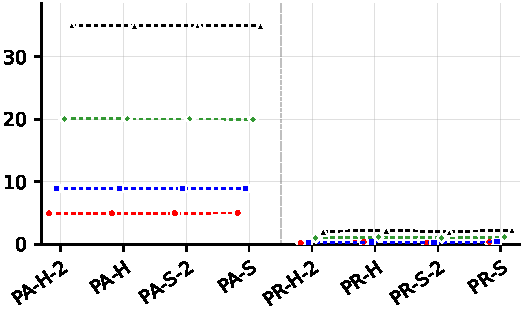
\includegraphics[width=\linewidth]{fig_rf_chd_49_pa_aabs.pdf}\\\scriptsize AABS (\ref{eq:aabs}) ($\downarrow$)\end{minipage} & \begin{minipage}{0.27\textwidth}\centering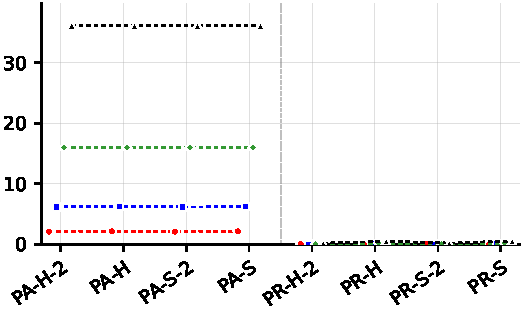
\includegraphics[width=\linewidth]{fig_rf_yeast_pa_aabs.pdf}\\\scriptsize AABS (\ref{eq:aabs}) ($\downarrow$)\end{minipage} & \begin{minipage}{0.27\textwidth}\centering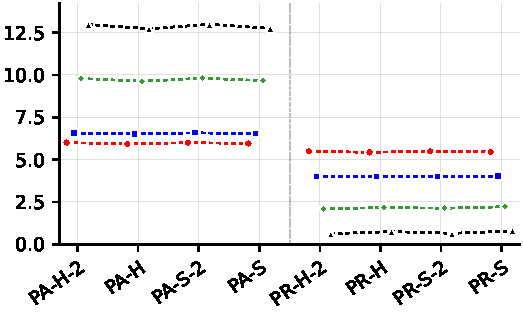
\includegraphics[width=\linewidth]{fig_rf_enron_pa_aabs.pdf}\\\scriptsize AABS (\ref{eq:aabs}) ($\downarrow$)\end{minipage} \\[8pt]
\begin{minipage}{0.27\textwidth}\centering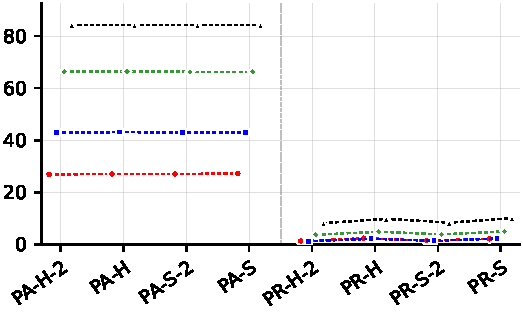
\includegraphics[width=\linewidth]{fig_rf_chd_49_pa_abs.pdf}\\\scriptsize ABS (\ref{eq:abs}) ($\downarrow$)\end{minipage} & \begin{minipage}{0.27\textwidth}\centering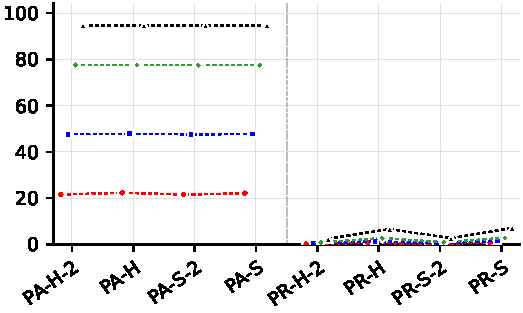
\includegraphics[width=\linewidth]{fig_rf_yeast_pa_abs.pdf}\\\scriptsize ABS (\ref{eq:abs}) ($\downarrow$)\end{minipage} & \begin{minipage}{0.27\textwidth}\centering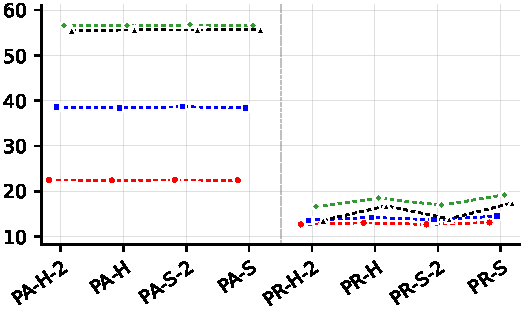
\includegraphics[width=\linewidth]{fig_rf_enron_pa_abs.pdf}\\\scriptsize ABS (\ref{eq:abs}) ($\downarrow$)\end{minipage} \\[8pt]
\end{tabular}
\caption{(Table G4) Average scores (in \%, $y$-axis) over $5\times 5$ cross-validation folds, plotted against the classifiers ($x$-axis): partial-order predictors (PA-H-2, PA-H, PA-S-2, PA-S) and preorder predictors (PR-H-2, PR-H, PR-S-2, PR-S). Results are color-coded with respect to the noisy level $\alpha$ as follows: \textcolor[HTML]{FF0000}{$\alpha = 0.0$}, \textcolor[HTML]{0000FF}{$\alpha = 0.1$}, \textcolor[HTML]{339933}{$\alpha = 0.2$} and \textcolor[HTML]{000000}{$\alpha = 0.3$}.}
\label{tab:paperapp_g4_rf_pa_g1}
\end{table}

\FloatBarrier

\pdfbookmark[3]{(Table G5) Group 1: emotions, scene, Water-quality}{paperapp_g5-rf-pa-g1}
\begin{table}[!htbp]
\centering
\setlength{\tabcolsep}{2pt}
\renewcommand{\arraystretch}{0.65}
\begin{tabular}{c!{\color{black!25}\vrule width 0.3pt}c!{\color{black!25}\vrule width 0.3pt}c}
\textbf{emotions} & \textbf{scene} & \textbf{Water-quality} \\
\begin{minipage}{0.27\textwidth}\centering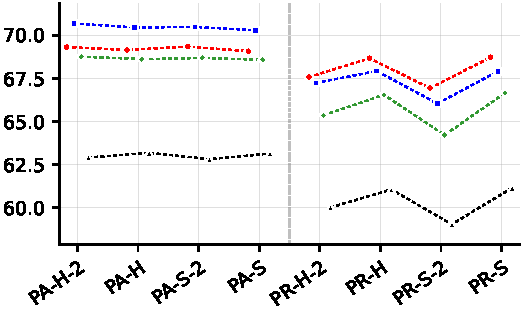
\includegraphics[width=\linewidth]{fig_rf_emotions_pa_f1_pa.pdf}\\\scriptsize $f^{1}_{\mathrm{MLC}}$ (\ref{eq:f1mlc}) ($\uparrow$)\end{minipage} & \begin{minipage}{0.27\textwidth}\centering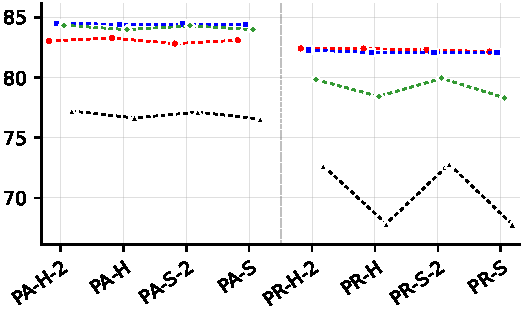
\includegraphics[width=\linewidth]{fig_rf_scene_pa_f1_pa.pdf}\\\scriptsize $f^{1}_{\mathrm{MLC}}$ (\ref{eq:f1mlc}) ($\uparrow$)\end{minipage} & \begin{minipage}{0.27\textwidth}\centering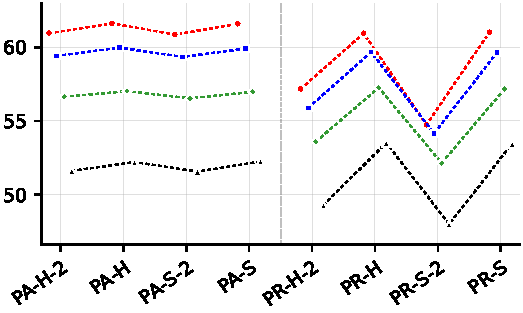
\includegraphics[width=\linewidth]{fig_rf_waterquality_pa_f1_pa.pdf}\\\scriptsize $f^{1}_{\mathrm{MLC}}$ (\ref{eq:f1mlc}) ($\uparrow$)\end{minipage} \\[8pt]
\begin{minipage}{0.27\textwidth}\centering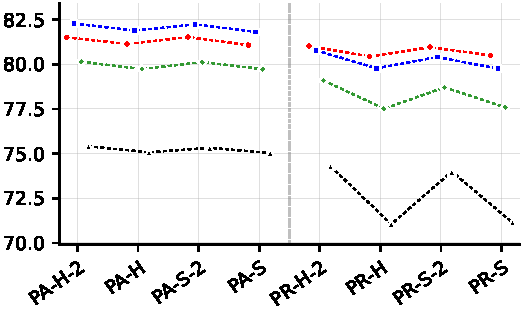
\includegraphics[width=\linewidth]{fig_rf_emotions_pa_hamming_accuracy_pa.pdf}\\\scriptsize $f^{\mathrm{ham}}_{\mathrm{MLC}}$ (\ref{eq:fham}) ($\uparrow$)\end{minipage} & \begin{minipage}{0.27\textwidth}\centering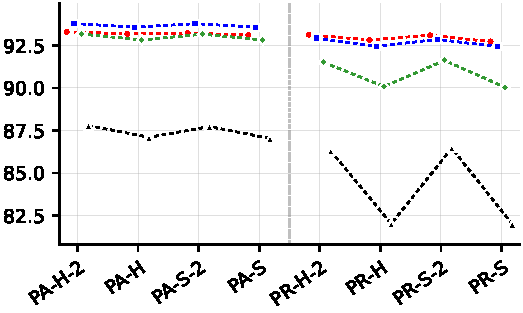
\includegraphics[width=\linewidth]{fig_rf_scene_pa_hamming_accuracy_pa.pdf}\\\scriptsize $f^{\mathrm{ham}}_{\mathrm{MLC}}$ (\ref{eq:fham}) ($\uparrow$)\end{minipage} & \begin{minipage}{0.27\textwidth}\centering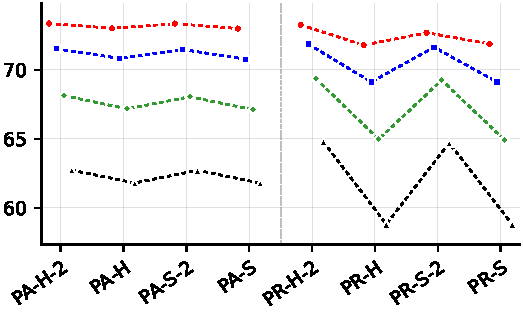
\includegraphics[width=\linewidth]{fig_rf_waterquality_pa_hamming_accuracy_pa.pdf}\\\scriptsize $f^{\mathrm{ham}}_{\mathrm{MLC}}$ (\ref{eq:fham}) ($\uparrow$)\end{minipage} \\[8pt]
\begin{minipage}{0.27\textwidth}\centering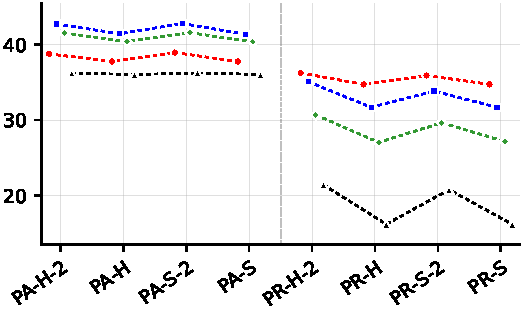
\includegraphics[width=\linewidth]{fig_rf_emotions_pa_subset0_1_pa.pdf}\\\scriptsize $f^{\mathrm{sub}}_{\mathrm{MLC}}$ (\ref{eq:fsub}) ($\uparrow$)\end{minipage} & \begin{minipage}{0.27\textwidth}\centering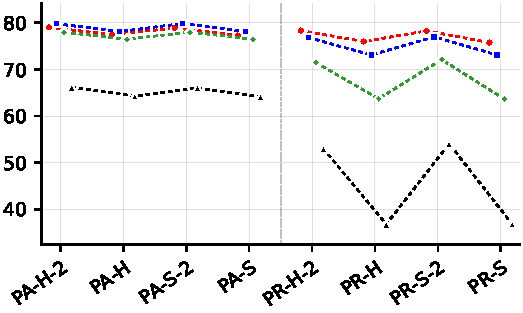
\includegraphics[width=\linewidth]{fig_rf_scene_pa_subset0_1_pa.pdf}\\\scriptsize $f^{\mathrm{sub}}_{\mathrm{MLC}}$ (\ref{eq:fsub}) ($\uparrow$)\end{minipage} & \begin{minipage}{0.27\textwidth}\centering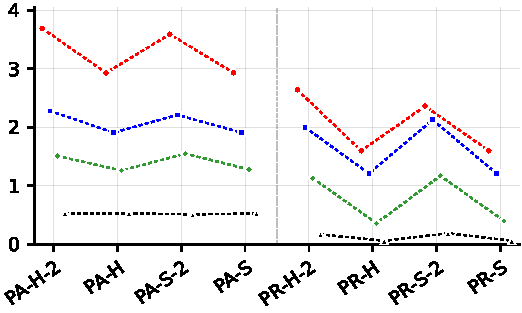
\includegraphics[width=\linewidth]{fig_rf_waterquality_pa_subset0_1_pa.pdf}\\\scriptsize $f^{\mathrm{sub}}_{\mathrm{MLC}}$ (\ref{eq:fsub}) ($\uparrow$)\end{minipage} \\[8pt]
\begin{minipage}{0.27\textwidth}\centering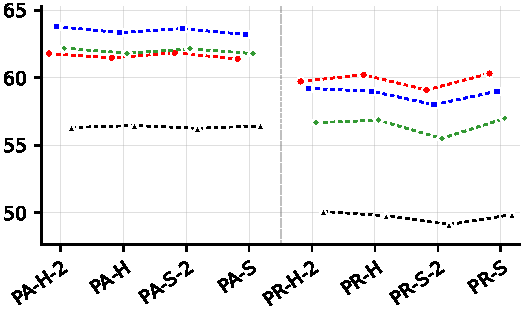
\includegraphics[width=\linewidth]{fig_rf_emotions_pa_jaccard_pa.pdf}\\\scriptsize $f^{\mathrm{Jacc}}_{\mathrm{MLC}}$ (\ref{eq:jaccmlc}) ($\uparrow$)\end{minipage} & \begin{minipage}{0.27\textwidth}\centering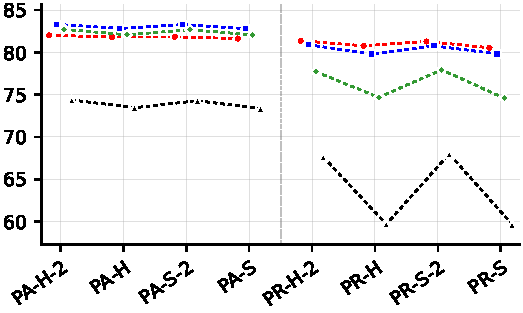
\includegraphics[width=\linewidth]{fig_rf_scene_pa_jaccard_pa.pdf}\\\scriptsize $f^{\mathrm{Jacc}}_{\mathrm{MLC}}$ (\ref{eq:jaccmlc}) ($\uparrow$)\end{minipage} & \begin{minipage}{0.27\textwidth}\centering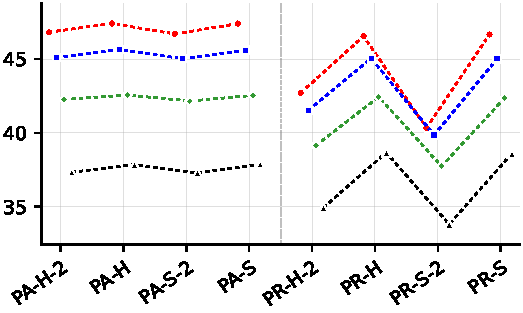
\includegraphics[width=\linewidth]{fig_rf_waterquality_pa_jaccard_pa.pdf}\\\scriptsize $f^{\mathrm{Jacc}}_{\mathrm{MLC}}$ (\ref{eq:jaccmlc}) ($\uparrow$)\end{minipage} \\[8pt]
\begin{minipage}{0.27\textwidth}\centering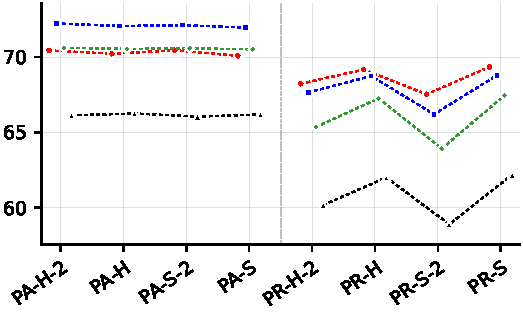
\includegraphics[width=\linewidth]{fig_rf_emotions_pa_macro_f1_pa.pdf}\\\scriptsize macro-$f_1$ (\ref{eq:macrof1}) ($\uparrow$)\end{minipage} & \begin{minipage}{0.27\textwidth}\centering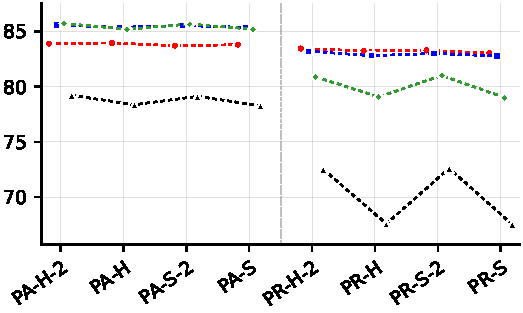
\includegraphics[width=\linewidth]{fig_rf_scene_pa_macro_f1_pa.pdf}\\\scriptsize macro-$f_1$ (\ref{eq:macrof1}) ($\uparrow$)\end{minipage} & \begin{minipage}{0.27\textwidth}\centering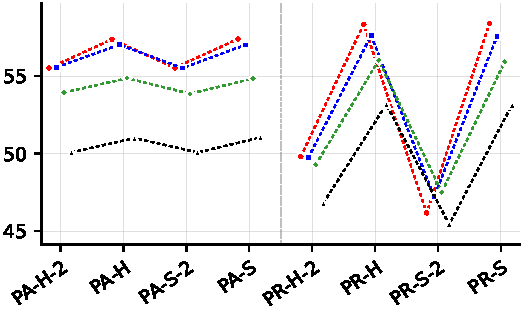
\includegraphics[width=\linewidth]{fig_rf_waterquality_pa_macro_f1_pa.pdf}\\\scriptsize macro-$f_1$ (\ref{eq:macrof1}) ($\uparrow$)\end{minipage} \\[8pt]
\begin{minipage}{0.27\textwidth}\centering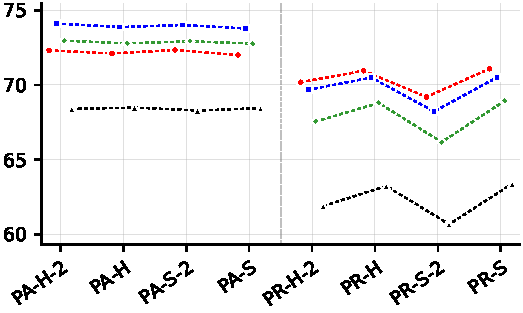
\includegraphics[width=\linewidth]{fig_rf_emotions_pa_micro_f1_pa.pdf}\\\scriptsize micro-$f_1$ (\ref{eq:microf1}) ($\uparrow$)\end{minipage} & \begin{minipage}{0.27\textwidth}\centering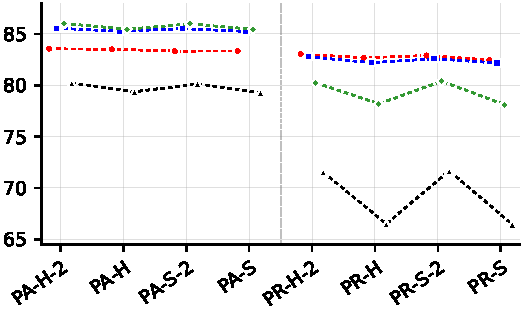
\includegraphics[width=\linewidth]{fig_rf_scene_pa_micro_f1_pa.pdf}\\\scriptsize micro-$f_1$ (\ref{eq:microf1}) ($\uparrow$)\end{minipage} & \begin{minipage}{0.27\textwidth}\centering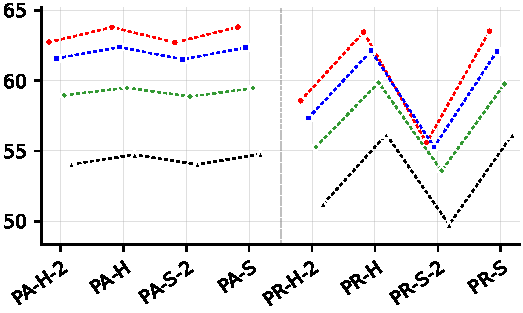
\includegraphics[width=\linewidth]{fig_rf_waterquality_pa_micro_f1_pa.pdf}\\\scriptsize micro-$f_1$ (\ref{eq:microf1}) ($\uparrow$)\end{minipage} \\[8pt]
\begin{minipage}{0.27\textwidth}\centering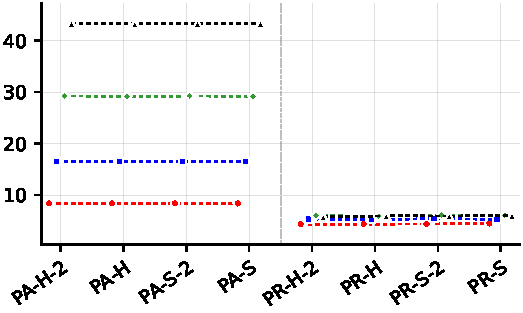
\includegraphics[width=\linewidth]{fig_rf_emotions_pa_aabs.pdf}\\\scriptsize AABS (\ref{eq:aabs}) ($\downarrow$)\end{minipage} & \begin{minipage}{0.27\textwidth}\centering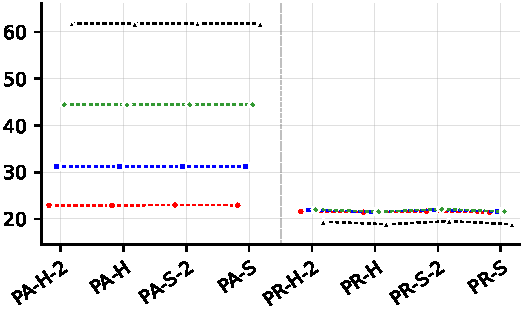
\includegraphics[width=\linewidth]{fig_rf_scene_pa_aabs.pdf}\\\scriptsize AABS (\ref{eq:aabs}) ($\downarrow$)\end{minipage} & \begin{minipage}{0.27\textwidth}\centering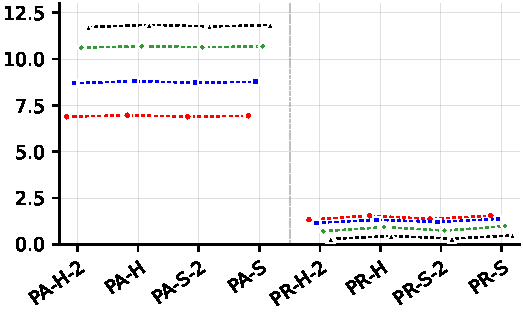
\includegraphics[width=\linewidth]{fig_rf_waterquality_pa_aabs.pdf}\\\scriptsize AABS (\ref{eq:aabs}) ($\downarrow$)\end{minipage} \\[8pt]
\begin{minipage}{0.27\textwidth}\centering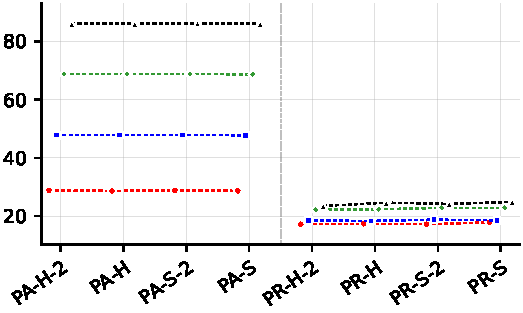
\includegraphics[width=\linewidth]{fig_rf_emotions_pa_abs.pdf}\\\scriptsize ABS (\ref{eq:abs}) ($\downarrow$)\end{minipage} & \begin{minipage}{0.27\textwidth}\centering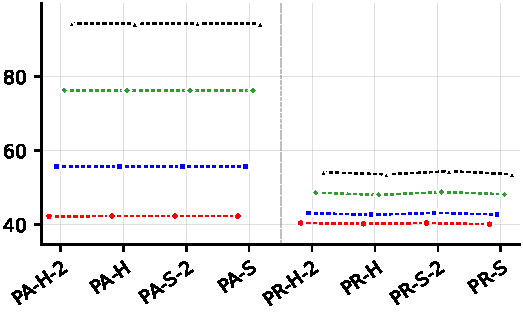
\includegraphics[width=\linewidth]{fig_rf_scene_pa_abs.pdf}\\\scriptsize ABS (\ref{eq:abs}) ($\downarrow$)\end{minipage} & \begin{minipage}{0.27\textwidth}\centering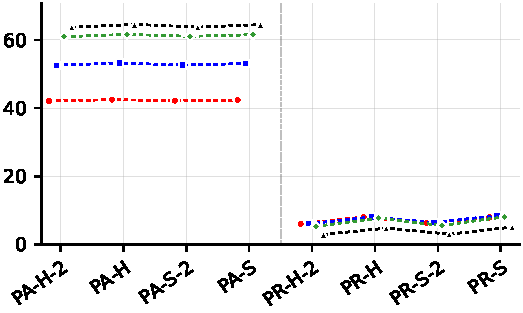
\includegraphics[width=\linewidth]{fig_rf_waterquality_pa_abs.pdf}\\\scriptsize ABS (\ref{eq:abs}) ($\downarrow$)\end{minipage} \\[8pt]
\end{tabular}
\caption{(Table G5) Average scores (in \%, $y$-axis) over $5\times 5$ cross-validation folds, plotted against the classifiers ($x$-axis): partial-order predictors (PA-H-2, PA-H, PA-S-2, PA-S) and preorder predictors (PR-H-2, PR-H, PR-S-2, PR-S). Results are color-coded with respect to the noisy level $\alpha$ as follows: \textcolor[HTML]{FF0000}{$\alpha = 0.0$}, \textcolor[HTML]{0000FF}{$\alpha = 0.1$}, \textcolor[HTML]{339933}{$\alpha = 0.2$} and \textcolor[HTML]{000000}{$\alpha = 0.3$}.}
\label{tab:paperapp_g5_rf_pa_g1}
\end{table}

\FloatBarrier

\subsubsection{Standard MLC predictions (BinaryVector)}

\pdfbookmark[3]{(Table G6) Group 1: GpositivePseAAC, PlantPseAAC, HumanPseAAC}{paperapp_g6-rf-bv-g1}
\begin{table}[!htbp]
\centering
\setlength{\tabcolsep}{2pt}
\renewcommand{\arraystretch}{0.65}
\begin{tabular}{c!{\color{black!25}\vrule width 0.3pt}c!{\color{black!25}\vrule width 0.3pt}c}
\textbf{GpositivePse} & \textbf{plantPse} & \textbf{HumanPse} \\
\begin{minipage}{0.27\textwidth}\centering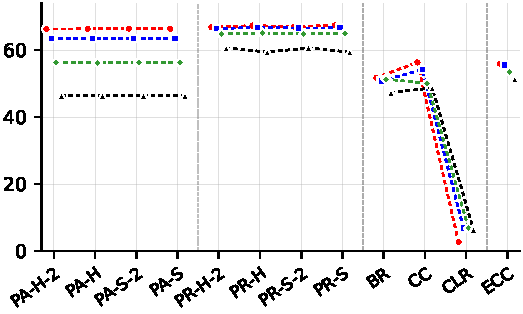
\includegraphics[width=\linewidth]{fig_rf_gpositivepseaac_bv_f1.pdf}\\\scriptsize $f^{1}_{\mathrm{MLC}}$ (\ref{eq:f1mlc}) ($\uparrow$)\end{minipage} & \begin{minipage}{0.27\textwidth}\centering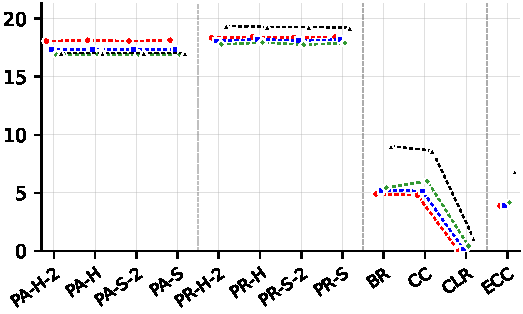
\includegraphics[width=\linewidth]{fig_rf_plantpseaac_bv_f1.pdf}\\\scriptsize $f^{1}_{\mathrm{MLC}}$ (\ref{eq:f1mlc}) ($\uparrow$)\end{minipage} & \begin{minipage}{0.27\textwidth}\centering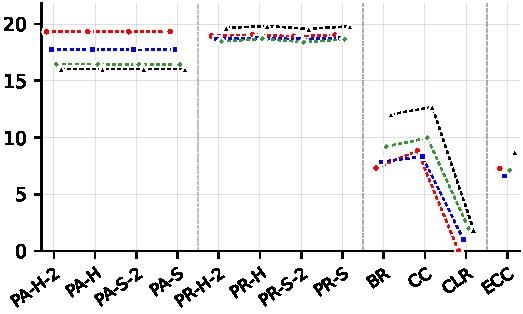
\includegraphics[width=\linewidth]{fig_rf_humanpseaac_bv_f1.pdf}\\\scriptsize $f^{1}_{\mathrm{MLC}}$ (\ref{eq:f1mlc}) ($\uparrow$)\end{minipage} \\[8pt]
\begin{minipage}{0.27\textwidth}\centering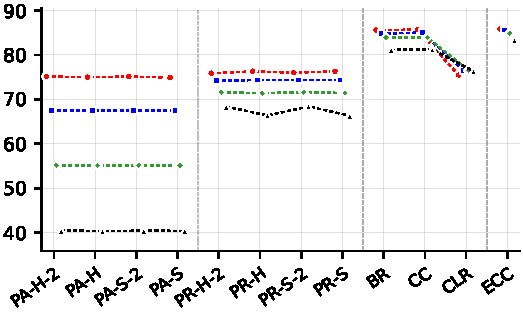
\includegraphics[width=\linewidth]{fig_rf_gpositivepseaac_bv_hamming_accuracy.pdf}\\\scriptsize $f^{\mathrm{ham}}_{\mathrm{MLC}}$ (\ref{eq:fham}) ($\uparrow$)\end{minipage} & \begin{minipage}{0.27\textwidth}\centering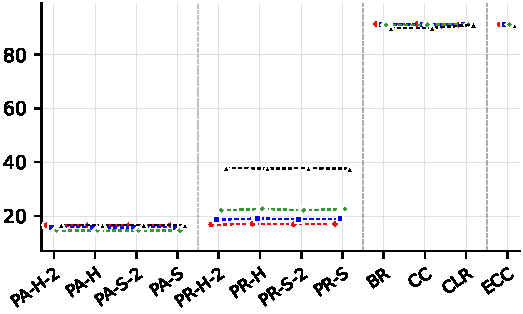
\includegraphics[width=\linewidth]{fig_rf_plantpseaac_bv_hamming_accuracy.pdf}\\\scriptsize $f^{\mathrm{ham}}_{\mathrm{MLC}}$ (\ref{eq:fham}) ($\uparrow$)\end{minipage} & \begin{minipage}{0.27\textwidth}\centering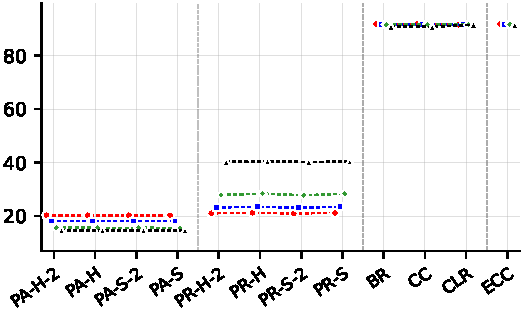
\includegraphics[width=\linewidth]{fig_rf_humanpseaac_bv_hamming_accuracy.pdf}\\\scriptsize $f^{\mathrm{ham}}_{\mathrm{MLC}}$ (\ref{eq:fham}) ($\uparrow$)\end{minipage} \\[8pt]
\begin{minipage}{0.27\textwidth}\centering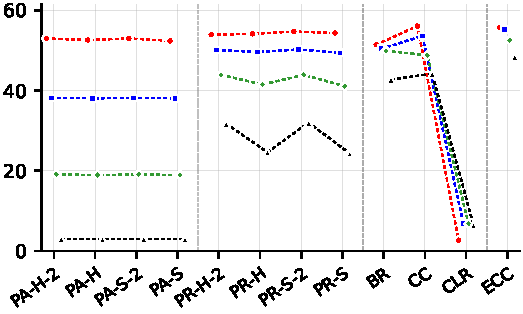
\includegraphics[width=\linewidth]{fig_rf_gpositivepseaac_bv_subset0_1.pdf}\\\scriptsize $f^{\mathrm{sub}}_{\mathrm{MLC}}$ (\ref{eq:fsub}) ($\uparrow$)\end{minipage} & \begin{minipage}{0.27\textwidth}\centering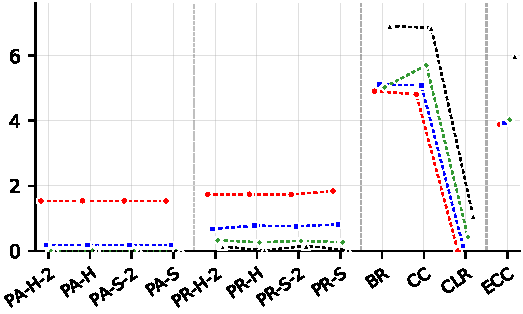
\includegraphics[width=\linewidth]{fig_rf_plantpseaac_bv_subset0_1.pdf}\\\scriptsize $f^{\mathrm{sub}}_{\mathrm{MLC}}$ (\ref{eq:fsub}) ($\uparrow$)\end{minipage} & \begin{minipage}{0.27\textwidth}\centering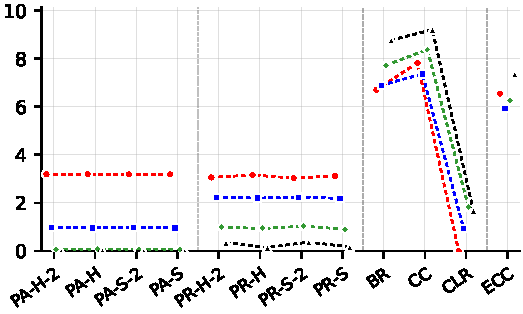
\includegraphics[width=\linewidth]{fig_rf_humanpseaac_bv_subset0_1.pdf}\\\scriptsize $f^{\mathrm{sub}}_{\mathrm{MLC}}$ (\ref{eq:fsub}) ($\uparrow$)\end{minipage} \\[8pt]
\begin{minipage}{0.27\textwidth}\centering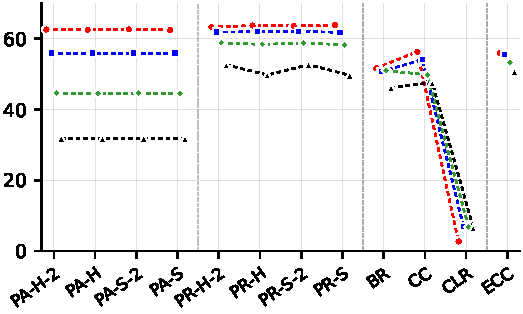
\includegraphics[width=\linewidth]{fig_rf_gpositivepseaac_bv_jaccard.pdf}\\\scriptsize $f^{\mathrm{Jacc}}_{\mathrm{MLC}}$ (\ref{eq:jaccmlc}) ($\uparrow$)\end{minipage} & \begin{minipage}{0.27\textwidth}\centering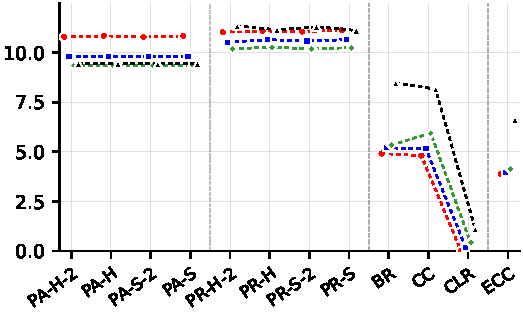
\includegraphics[width=\linewidth]{fig_rf_plantpseaac_bv_jaccard.pdf}\\\scriptsize $f^{\mathrm{Jacc}}_{\mathrm{MLC}}$ (\ref{eq:jaccmlc}) ($\uparrow$)\end{minipage} & \begin{minipage}{0.27\textwidth}\centering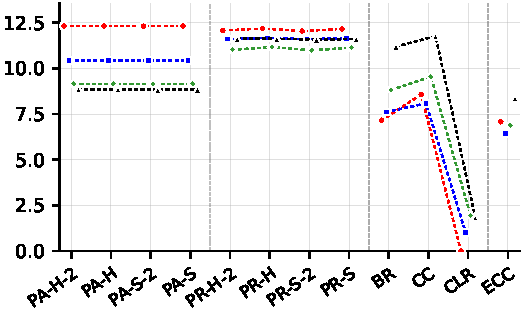
\includegraphics[width=\linewidth]{fig_rf_humanpseaac_bv_jaccard.pdf}\\\scriptsize $f^{\mathrm{Jacc}}_{\mathrm{MLC}}$ (\ref{eq:jaccmlc}) ($\uparrow$)\end{minipage} \\[8pt]
\begin{minipage}{0.27\textwidth}\centering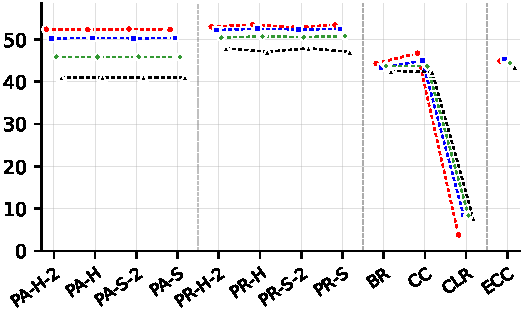
\includegraphics[width=\linewidth]{fig_rf_gpositivepseaac_bv_macro_f1.pdf}\\\scriptsize macro-$f_1$ (\ref{eq:macrof1}) ($\uparrow$)\end{minipage} & \begin{minipage}{0.27\textwidth}\centering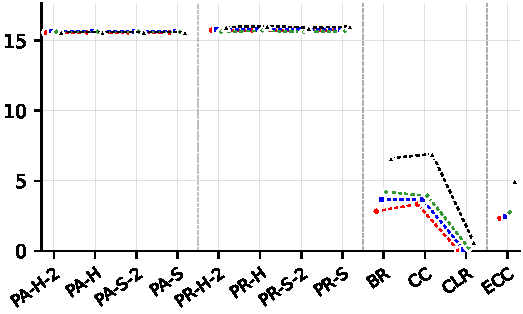
\includegraphics[width=\linewidth]{fig_rf_plantpseaac_bv_macro_f1.pdf}\\\scriptsize macro-$f_1$ (\ref{eq:macrof1}) ($\uparrow$)\end{minipage} & \begin{minipage}{0.27\textwidth}\centering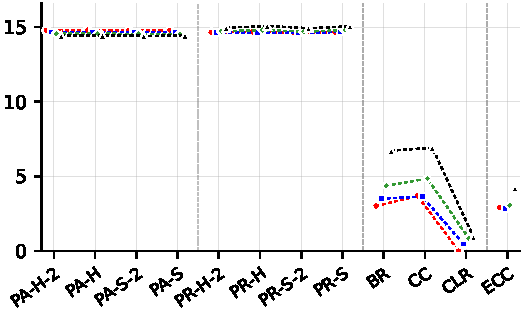
\includegraphics[width=\linewidth]{fig_rf_humanpseaac_bv_macro_f1.pdf}\\\scriptsize macro-$f_1$ (\ref{eq:macrof1}) ($\uparrow$)\end{minipage} \\[8pt]
\begin{minipage}{0.27\textwidth}\centering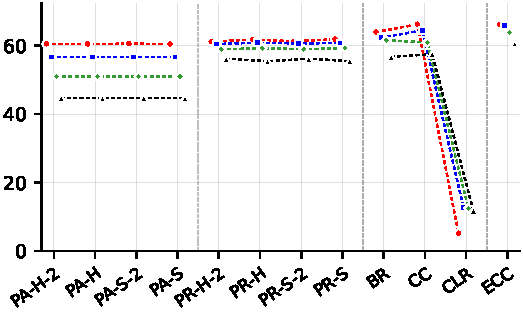
\includegraphics[width=\linewidth]{fig_rf_gpositivepseaac_bv_micro_f1.pdf}\\\scriptsize micro-$f_1$ (\ref{eq:microf1}) ($\uparrow$)\end{minipage} & \begin{minipage}{0.27\textwidth}\centering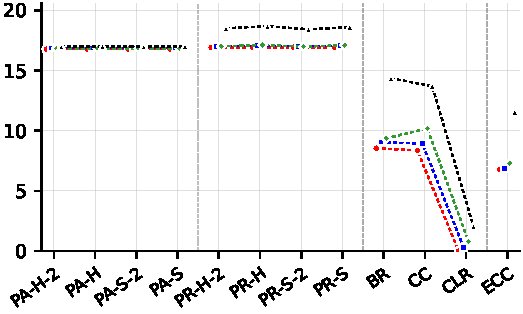
\includegraphics[width=\linewidth]{fig_rf_plantpseaac_bv_micro_f1.pdf}\\\scriptsize micro-$f_1$ (\ref{eq:microf1}) ($\uparrow$)\end{minipage} & \begin{minipage}{0.27\textwidth}\centering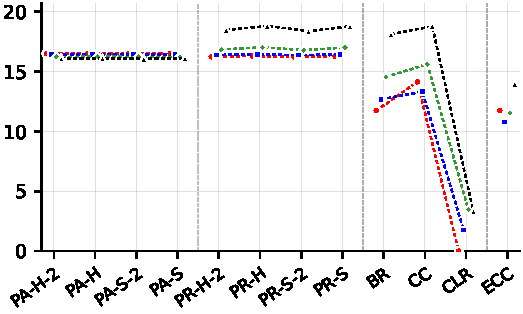
\includegraphics[width=\linewidth]{fig_rf_humanpseaac_bv_micro_f1.pdf}\\\scriptsize micro-$f_1$ (\ref{eq:microf1}) ($\uparrow$)\end{minipage} \\[8pt]
\begin{minipage}{0.27\textwidth}\centering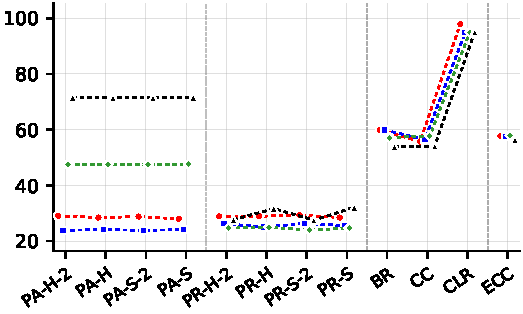
\includegraphics[width=\linewidth]{fig_rf_gpositivepseaac_bv_afrd.pdf}\\\scriptsize AFRD (\ref{eq:afrd}) ($\downarrow$)\end{minipage} & \begin{minipage}{0.27\textwidth}\centering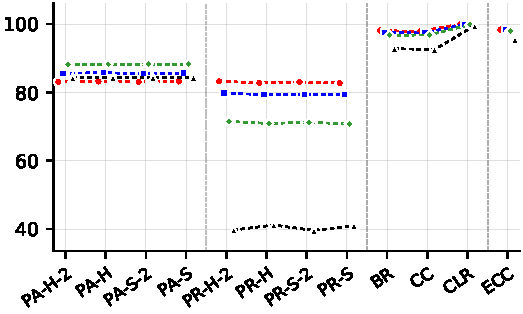
\includegraphics[width=\linewidth]{fig_rf_plantpseaac_bv_afrd.pdf}\\\scriptsize AFRD (\ref{eq:afrd}) ($\downarrow$)\end{minipage} & \begin{minipage}{0.27\textwidth}\centering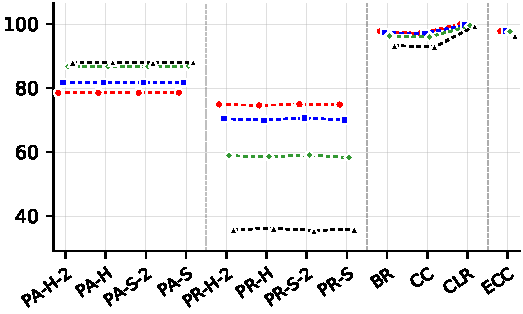
\includegraphics[width=\linewidth]{fig_rf_humanpseaac_bv_afrd.pdf}\\\scriptsize AFRD (\ref{eq:afrd}) ($\downarrow$)\end{minipage} \\[8pt]
\begin{minipage}{0.27\textwidth}\centering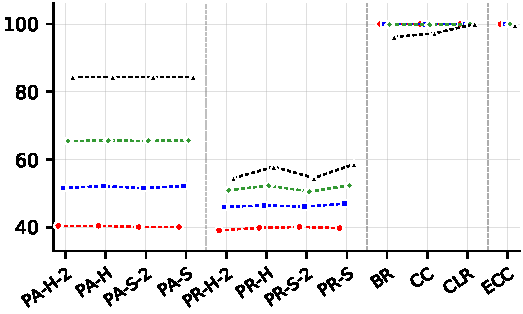
\includegraphics[width=\linewidth]{fig_rf_gpositivepseaac_bv_mfrd.pdf}\\\scriptsize MFRD (\ref{eq:mfrd}) ($\downarrow$)\end{minipage} & \begin{minipage}{0.27\textwidth}\centering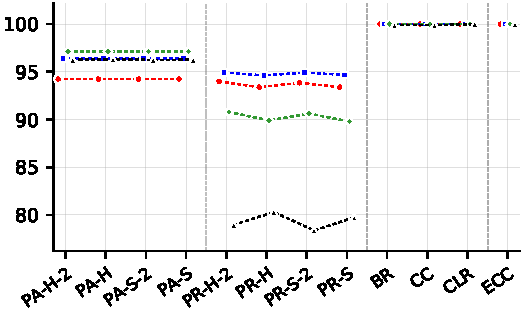
\includegraphics[width=\linewidth]{fig_rf_plantpseaac_bv_mfrd.pdf}\\\scriptsize MFRD (\ref{eq:mfrd}) ($\downarrow$)\end{minipage} & \begin{minipage}{0.27\textwidth}\centering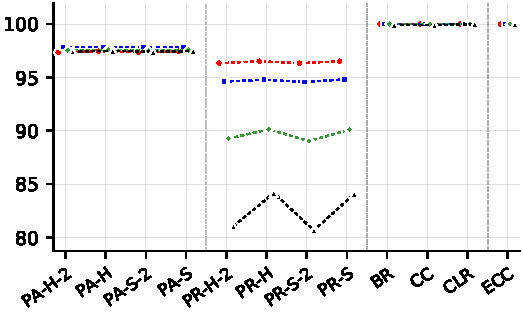
\includegraphics[width=\linewidth]{fig_rf_humanpseaac_bv_mfrd.pdf}\\\scriptsize MFRD (\ref{eq:mfrd}) ($\downarrow$)\end{minipage} \\[8pt]
\end{tabular}
\caption{(Table G6) Average scores (in \%, $y$-axis) over $5\times 5$ cross-validation folds, plotted against the classifiers ($x$-axis): partial-order predictors (PA-H-2, PA-H, PA-S-2, PA-S), preorder predictors (PR-H-2, PR-H, PR-S-2, PR-S), and standard MLC baselines (BR, CC, CLR). Results are color-coded with respect to the noisy level $\alpha$ as follows: \textcolor[HTML]{FF0000}{$\alpha = 0.0$}, \textcolor[HTML]{0000FF}{$\alpha = 0.1$}, \textcolor[HTML]{339933}{$\alpha = 0.2$} and \textcolor[HTML]{000000}{$\alpha = 0.3$}.}
\label{tab:paperapp_g6_rf_bv_g1}
\end{table}

\FloatBarrier

\subsubsection{Partial abstention (PartialAbstention)}

\pdfbookmark[3]{(Table G7) Group 1: GpositivePseAAC, PlantPseAAC, HumanPseAAC}{paperapp_g7-rf-pa-g1}
\begin{table}[!htbp]
\centering
\setlength{\tabcolsep}{2pt}
\renewcommand{\arraystretch}{0.65}
\begin{tabular}{c!{\color{black!25}\vrule width 0.3pt}c!{\color{black!25}\vrule width 0.3pt}c}
\textbf{GpositivePse} & \textbf{plantPse} & \textbf{HumanPse} \\
\begin{minipage}{0.27\textwidth}\centering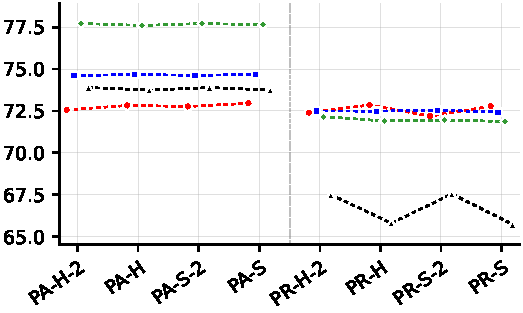
\includegraphics[width=\linewidth]{fig_rf_gpositivepseaac_pa_f1_pa.pdf}\\\scriptsize $f^{1}_{\mathrm{MLC}}$ (\ref{eq:f1mlc}) ($\uparrow$)\end{minipage} & \begin{minipage}{0.27\textwidth}\centering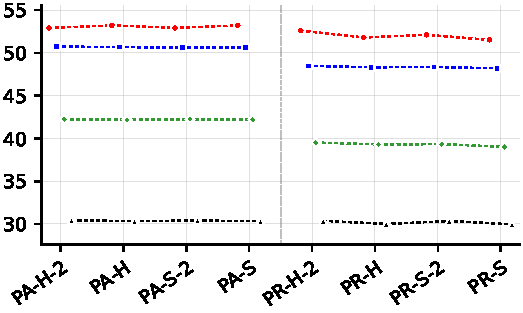
\includegraphics[width=\linewidth]{fig_rf_plantpseaac_pa_f1_pa.pdf}\\\scriptsize $f^{1}_{\mathrm{MLC}}$ (\ref{eq:f1mlc}) ($\uparrow$)\end{minipage} & \begin{minipage}{0.27\textwidth}\centering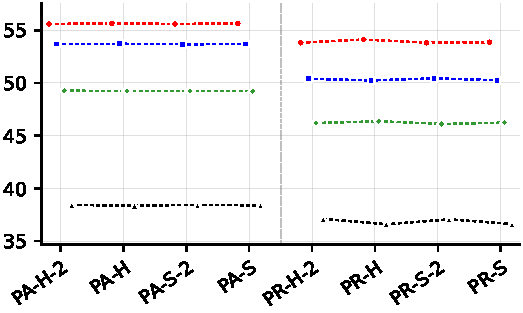
\includegraphics[width=\linewidth]{fig_rf_humanpseaac_pa_f1_pa.pdf}\\\scriptsize $f^{1}_{\mathrm{MLC}}$ (\ref{eq:f1mlc}) ($\uparrow$)\end{minipage} \\[8pt]
\begin{minipage}{0.27\textwidth}\centering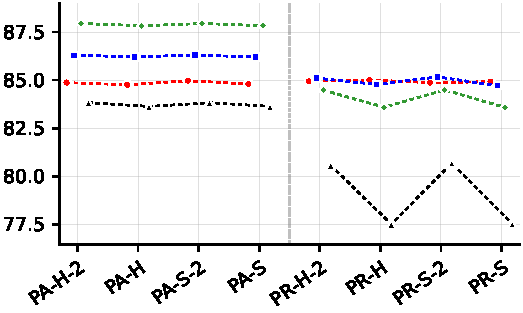
\includegraphics[width=\linewidth]{fig_rf_gpositivepseaac_pa_hamming_accuracy_pa.pdf}\\\scriptsize $f^{\mathrm{ham}}_{\mathrm{MLC}}$ (\ref{eq:fham}) ($\uparrow$)\end{minipage} & \begin{minipage}{0.27\textwidth}\centering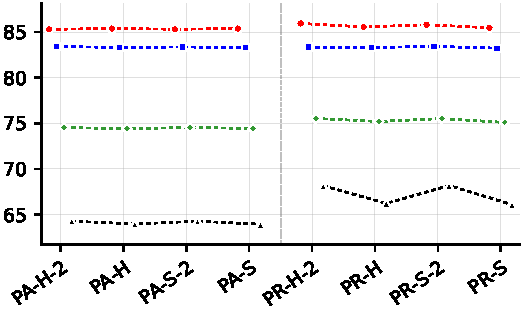
\includegraphics[width=\linewidth]{fig_rf_plantpseaac_pa_hamming_accuracy_pa.pdf}\\\scriptsize $f^{\mathrm{ham}}_{\mathrm{MLC}}$ (\ref{eq:fham}) ($\uparrow$)\end{minipage} & \begin{minipage}{0.27\textwidth}\centering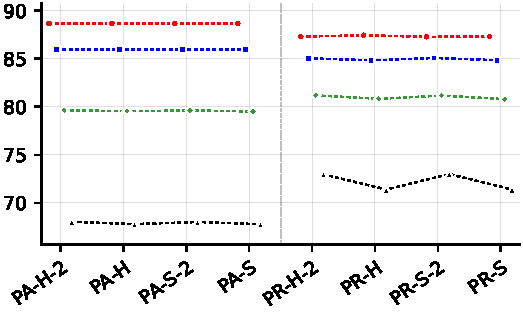
\includegraphics[width=\linewidth]{fig_rf_humanpseaac_pa_hamming_accuracy_pa.pdf}\\\scriptsize $f^{\mathrm{ham}}_{\mathrm{MLC}}$ (\ref{eq:fham}) ($\uparrow$)\end{minipage} \\[8pt]
\begin{minipage}{0.27\textwidth}\centering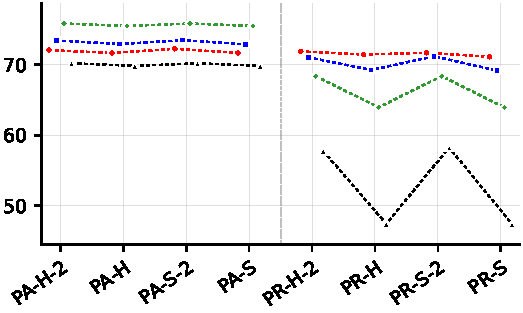
\includegraphics[width=\linewidth]{fig_rf_gpositivepseaac_pa_subset0_1_pa.pdf}\\\scriptsize $f^{\mathrm{sub}}_{\mathrm{MLC}}$ (\ref{eq:fsub}) ($\uparrow$)\end{minipage} & \begin{minipage}{0.27\textwidth}\centering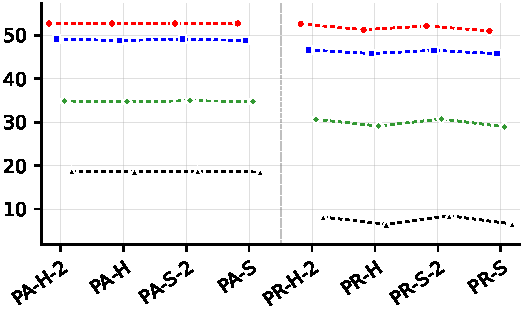
\includegraphics[width=\linewidth]{fig_rf_plantpseaac_pa_subset0_1_pa.pdf}\\\scriptsize $f^{\mathrm{sub}}_{\mathrm{MLC}}$ (\ref{eq:fsub}) ($\uparrow$)\end{minipage} & \begin{minipage}{0.27\textwidth}\centering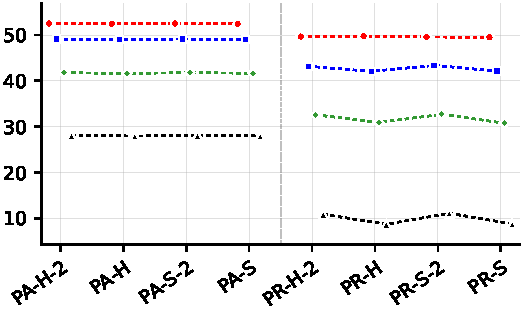
\includegraphics[width=\linewidth]{fig_rf_humanpseaac_pa_subset0_1_pa.pdf}\\\scriptsize $f^{\mathrm{sub}}_{\mathrm{MLC}}$ (\ref{eq:fsub}) ($\uparrow$)\end{minipage} \\[8pt]
\begin{minipage}{0.27\textwidth}\centering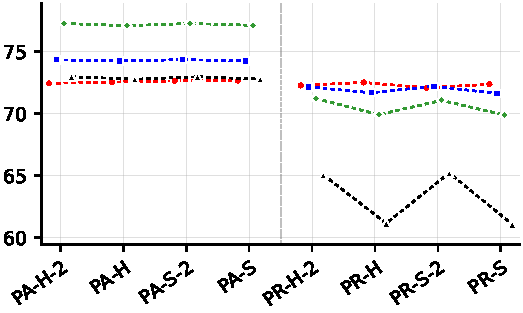
\includegraphics[width=\linewidth]{fig_rf_gpositivepseaac_pa_jaccard_pa.pdf}\\\scriptsize $f^{\mathrm{Jacc}}_{\mathrm{MLC}}$ (\ref{eq:jaccmlc}) ($\uparrow$)\end{minipage} & \begin{minipage}{0.27\textwidth}\centering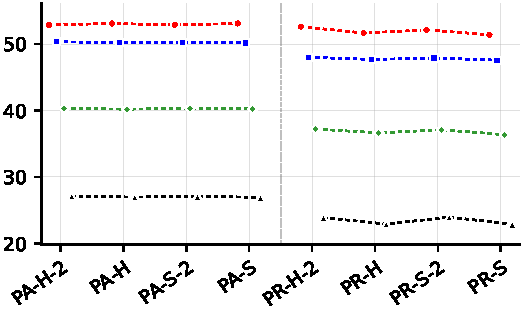
\includegraphics[width=\linewidth]{fig_rf_plantpseaac_pa_jaccard_pa.pdf}\\\scriptsize $f^{\mathrm{Jacc}}_{\mathrm{MLC}}$ (\ref{eq:jaccmlc}) ($\uparrow$)\end{minipage} & \begin{minipage}{0.27\textwidth}\centering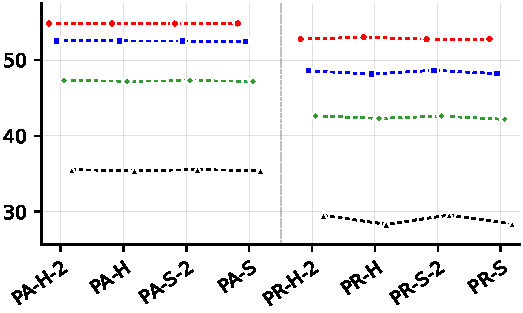
\includegraphics[width=\linewidth]{fig_rf_humanpseaac_pa_jaccard_pa.pdf}\\\scriptsize $f^{\mathrm{Jacc}}_{\mathrm{MLC}}$ (\ref{eq:jaccmlc}) ($\uparrow$)\end{minipage} \\[8pt]
\begin{minipage}{0.27\textwidth}\centering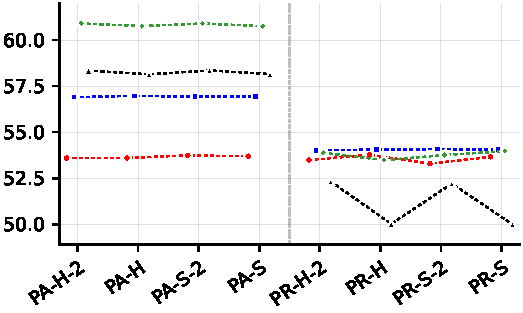
\includegraphics[width=\linewidth]{fig_rf_gpositivepseaac_pa_macro_f1_pa.pdf}\\\scriptsize macro-$f_1$ (\ref{eq:macrof1}) ($\uparrow$)\end{minipage} & \begin{minipage}{0.27\textwidth}\centering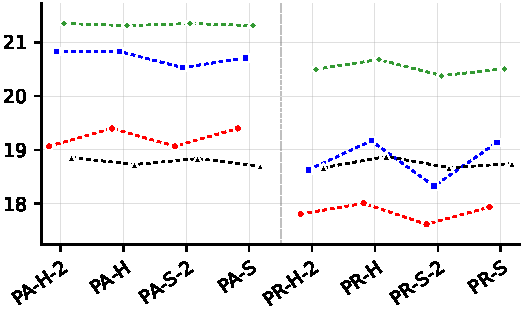
\includegraphics[width=\linewidth]{fig_rf_plantpseaac_pa_macro_f1_pa.pdf}\\\scriptsize macro-$f_1$ (\ref{eq:macrof1}) ($\uparrow$)\end{minipage} & \begin{minipage}{0.27\textwidth}\centering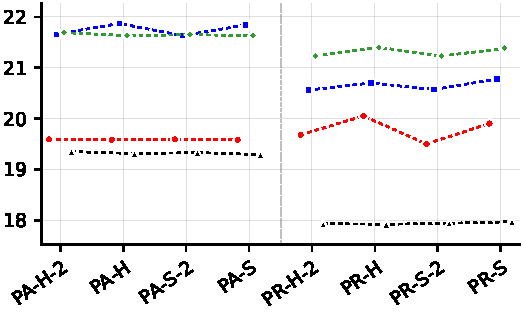
\includegraphics[width=\linewidth]{fig_rf_humanpseaac_pa_macro_f1_pa.pdf}\\\scriptsize macro-$f_1$ (\ref{eq:macrof1}) ($\uparrow$)\end{minipage} \\[8pt]
\begin{minipage}{0.27\textwidth}\centering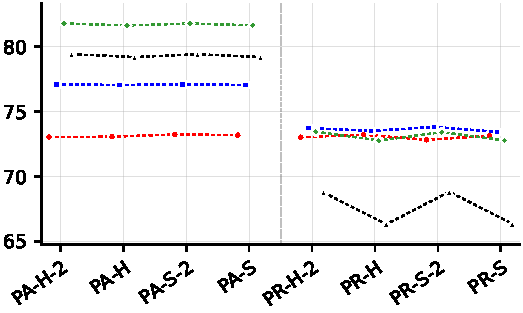
\includegraphics[width=\linewidth]{fig_rf_gpositivepseaac_pa_micro_f1_pa.pdf}\\\scriptsize micro-$f_1$ (\ref{eq:microf1}) ($\uparrow$)\end{minipage} & \begin{minipage}{0.27\textwidth}\centering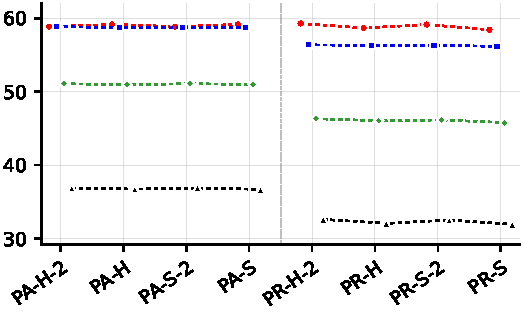
\includegraphics[width=\linewidth]{fig_rf_plantpseaac_pa_micro_f1_pa.pdf}\\\scriptsize micro-$f_1$ (\ref{eq:microf1}) ($\uparrow$)\end{minipage} & \begin{minipage}{0.27\textwidth}\centering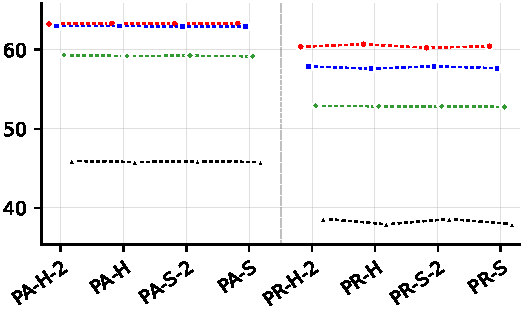
\includegraphics[width=\linewidth]{fig_rf_humanpseaac_pa_micro_f1_pa.pdf}\\\scriptsize micro-$f_1$ (\ref{eq:microf1}) ($\uparrow$)\end{minipage} \\[8pt]
\begin{minipage}{0.27\textwidth}\centering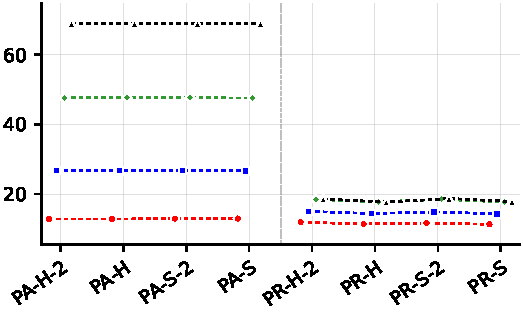
\includegraphics[width=\linewidth]{fig_rf_gpositivepseaac_pa_aabs.pdf}\\\scriptsize AABS (\ref{eq:aabs}) ($\downarrow$)\end{minipage} & \begin{minipage}{0.27\textwidth}\centering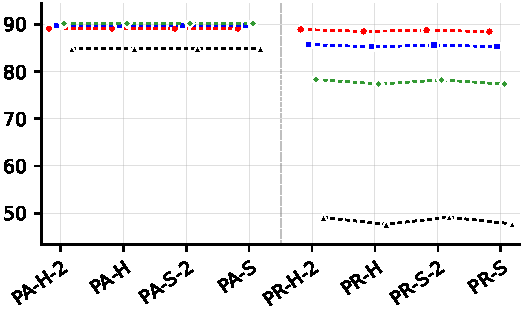
\includegraphics[width=\linewidth]{fig_rf_plantpseaac_pa_aabs.pdf}\\\scriptsize AABS (\ref{eq:aabs}) ($\downarrow$)\end{minipage} & \begin{minipage}{0.27\textwidth}\centering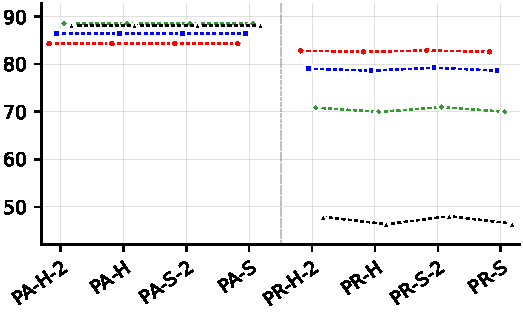
\includegraphics[width=\linewidth]{fig_rf_humanpseaac_pa_aabs.pdf}\\\scriptsize AABS (\ref{eq:aabs}) ($\downarrow$)\end{minipage} \\[8pt]
\begin{minipage}{0.27\textwidth}\centering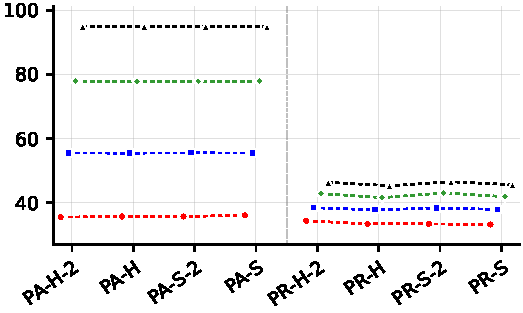
\includegraphics[width=\linewidth]{fig_rf_gpositivepseaac_pa_abs.pdf}\\\scriptsize ABS (\ref{eq:abs}) ($\downarrow$)\end{minipage} & \begin{minipage}{0.27\textwidth}\centering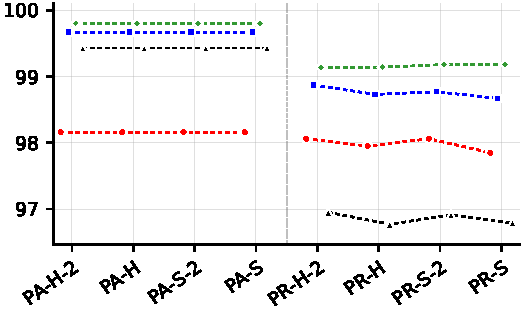
\includegraphics[width=\linewidth]{fig_rf_plantpseaac_pa_abs.pdf}\\\scriptsize ABS (\ref{eq:abs}) ($\downarrow$)\end{minipage} & \begin{minipage}{0.27\textwidth}\centering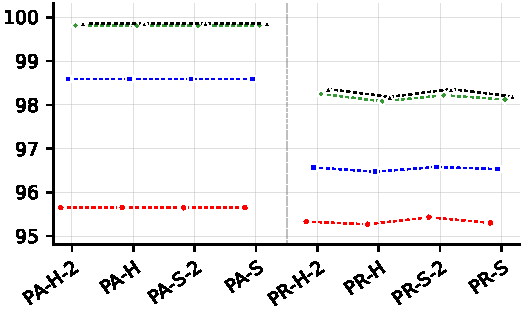
\includegraphics[width=\linewidth]{fig_rf_humanpseaac_pa_abs.pdf}\\\scriptsize ABS (\ref{eq:abs}) ($\downarrow$)\end{minipage} \\[8pt]
\end{tabular}
\caption{(Table G7) Average scores (in \%, $y$-axis) over $5\times 5$ cross-validation folds, plotted against the classifiers ($x$-axis): partial-order predictors (PA-H-2, PA-H, PA-S-2, PA-S) and preorder predictors (PR-H-2, PR-H, PR-S-2, PR-S). Results are color-coded with respect to the noisy level $\alpha$ as follows: \textcolor[HTML]{FF0000}{$\alpha = 0.0$}, \textcolor[HTML]{0000FF}{$\alpha = 0.1$}, \textcolor[HTML]{339933}{$\alpha = 0.2$} and \textcolor[HTML]{000000}{$\alpha = 0.3$}.}
\label{tab:paperapp_g7_rf_pa_g1}
\end{table}

\FloatBarrier

\subsubsection{Standard MLC predictions (BinaryVector)}

\pdfbookmark[3]{(Table G8) VirusPseAAC}{paperapp_g8-rf-bv-g1}
\begin{table}[!htbp]
\centering
\setlength{\tabcolsep}{2pt}
\renewcommand{\arraystretch}{0.65}
\begin{tabular}{c}
\textbf{VirusPseAAC} \\
\begin{minipage}{0.40\textwidth}\centering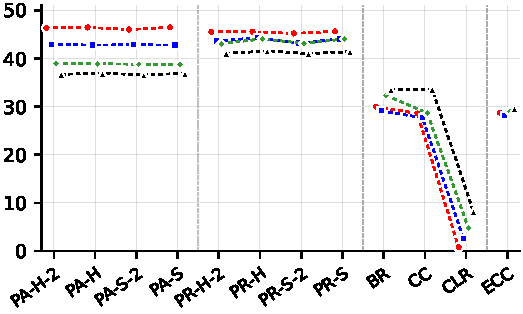
\includegraphics[width=\linewidth]{fig_rf_viruspseaac_bv_f1.pdf}\\\scriptsize $f^{1}_{\mathrm{MLC}}$ (\ref{eq:f1mlc}) ($\uparrow$)\end{minipage} \\[8pt]
\begin{minipage}{0.40\textwidth}\centering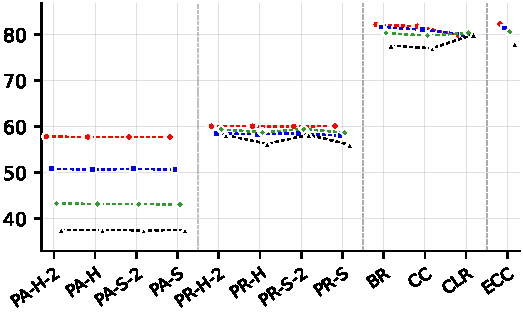
\includegraphics[width=\linewidth]{fig_rf_viruspseaac_bv_hamming_accuracy.pdf}\\\scriptsize $f^{\mathrm{ham}}_{\mathrm{MLC}}$ (\ref{eq:fham}) ($\uparrow$)\end{minipage} \\[8pt]
\begin{minipage}{0.40\textwidth}\centering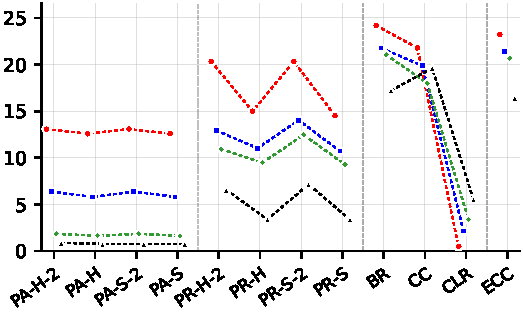
\includegraphics[width=\linewidth]{fig_rf_viruspseaac_bv_subset0_1.pdf}\\\scriptsize $f^{\mathrm{sub}}_{\mathrm{MLC}}$ (\ref{eq:fsub}) ($\uparrow$)\end{minipage} \\[8pt]
\begin{minipage}{0.40\textwidth}\centering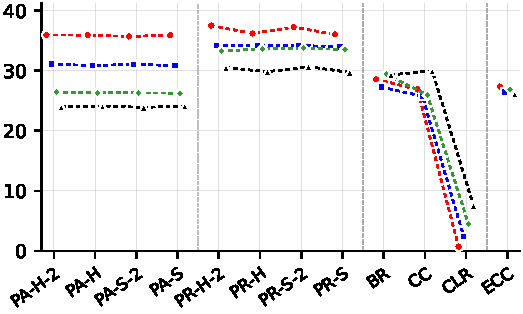
\includegraphics[width=\linewidth]{fig_rf_viruspseaac_bv_jaccard.pdf}\\\scriptsize $f^{\mathrm{Jacc}}_{\mathrm{MLC}}$ (\ref{eq:jaccmlc}) ($\uparrow$)\end{minipage} \\[8pt]
\begin{minipage}{0.40\textwidth}\centering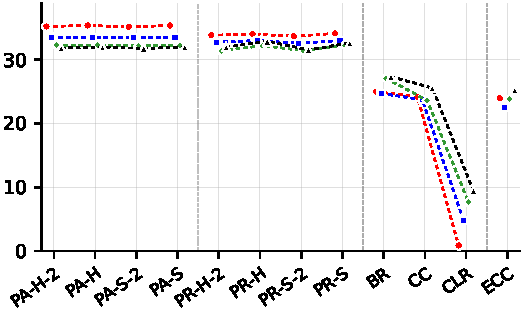
\includegraphics[width=\linewidth]{fig_rf_viruspseaac_bv_macro_f1.pdf}\\\scriptsize macro-$f_1$ (\ref{eq:macrof1}) ($\uparrow$)\end{minipage} \\[8pt]
\begin{minipage}{0.40\textwidth}\centering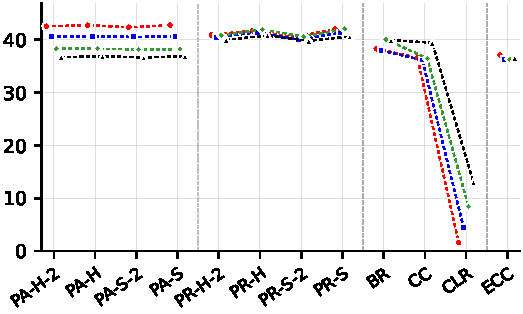
\includegraphics[width=\linewidth]{fig_rf_viruspseaac_bv_micro_f1.pdf}\\\scriptsize micro-$f_1$ (\ref{eq:microf1}) ($\uparrow$)\end{minipage} \\[8pt]
\begin{minipage}{0.40\textwidth}\centering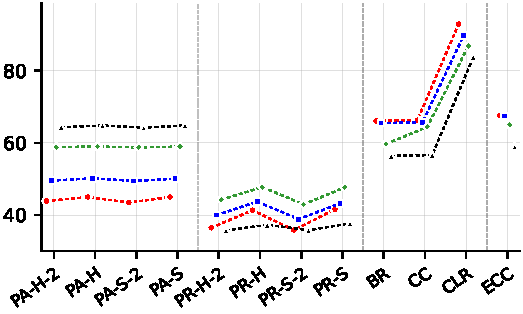
\includegraphics[width=\linewidth]{fig_rf_viruspseaac_bv_afrd.pdf}\\\scriptsize AFRD (\ref{eq:afrd}) ($\downarrow$)\end{minipage} \\[8pt]
\begin{minipage}{0.40\textwidth}\centering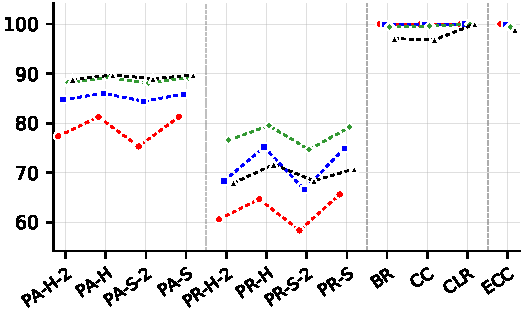
\includegraphics[width=\linewidth]{fig_rf_viruspseaac_bv_mfrd.pdf}\\\scriptsize MFRD (\ref{eq:mfrd}) ($\downarrow$)\end{minipage} \\[8pt]
\end{tabular}
\caption{(Table G8) VirusPseAAC --- average scores (in \%, $y$-axis) over $5\times 5$ cross-validation folds, plotted against the classifiers ($x$-axis): partial-order predictors (PA-H-2, PA-H, PA-S-2, PA-S), preorder predictors (PR-H-2, PR-H, PR-S-2, PR-S), and standard MLC baselines (BR, CC, CLR). Results are color-coded with respect to the noisy level $\alpha$ as follows: \textcolor[HTML]{FF0000}{$\alpha = 0.0$}, \textcolor[HTML]{0000FF}{$\alpha = 0.1$}, \textcolor[HTML]{339933}{$\alpha = 0.2$} and \textcolor[HTML]{000000}{$\alpha = 0.3$}.}
\label{tab:paperapp_g8_rf_bv_g1}
\end{table}

\FloatBarrier

\subsubsection{Partial abstention (PartialAbstention)}

\pdfbookmark[3]{(Table G9) VirusPseAAC}{paperapp_g9-rf-pa-g1}
\begin{table}[!htbp]
\centering
\setlength{\tabcolsep}{2pt}
\renewcommand{\arraystretch}{0.65}
\begin{tabular}{c}
\textbf{VirusPseAAC} \\
\begin{minipage}{0.40\textwidth}\centering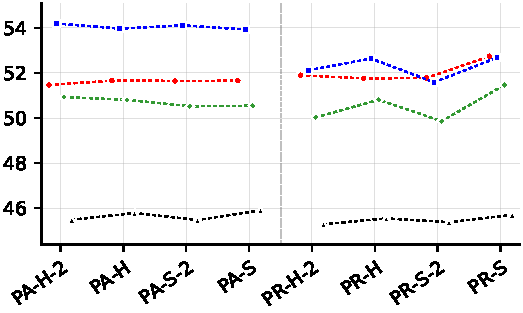
\includegraphics[width=\linewidth]{fig_rf_viruspseaac_pa_f1_pa.pdf}\\\scriptsize $f^{1}_{\mathrm{MLC}}$ (\ref{eq:f1mlc}) ($\uparrow$)\end{minipage} \\[8pt]
\begin{minipage}{0.40\textwidth}\centering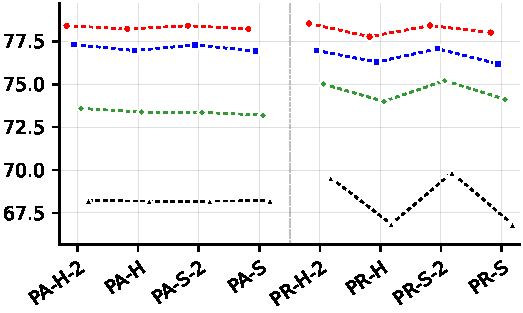
\includegraphics[width=\linewidth]{fig_rf_viruspseaac_pa_hamming_accuracy_pa.pdf}\\\scriptsize $f^{\mathrm{ham}}_{\mathrm{MLC}}$ (\ref{eq:fham}) ($\uparrow$)\end{minipage} \\[8pt]
\begin{minipage}{0.40\textwidth}\centering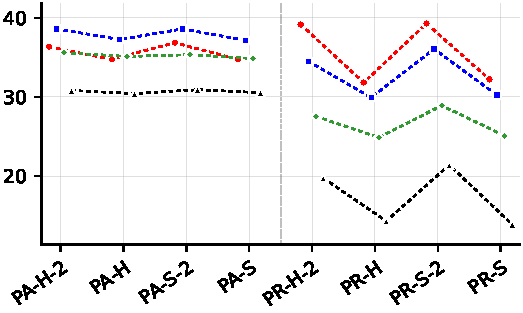
\includegraphics[width=\linewidth]{fig_rf_viruspseaac_pa_subset0_1_pa.pdf}\\\scriptsize $f^{\mathrm{sub}}_{\mathrm{MLC}}$ (\ref{eq:fsub}) ($\uparrow$)\end{minipage} \\[8pt]
\begin{minipage}{0.40\textwidth}\centering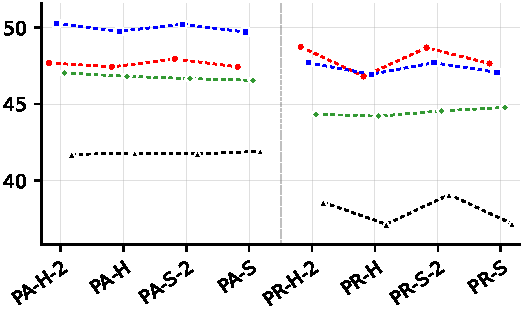
\includegraphics[width=\linewidth]{fig_rf_viruspseaac_pa_jaccard_pa.pdf}\\\scriptsize $f^{\mathrm{Jacc}}_{\mathrm{MLC}}$ (\ref{eq:jaccmlc}) ($\uparrow$)\end{minipage} \\[8pt]
\begin{minipage}{0.40\textwidth}\centering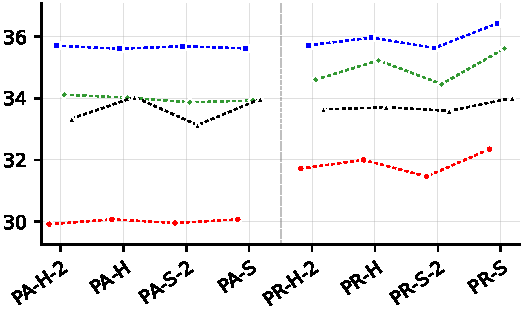
\includegraphics[width=\linewidth]{fig_rf_viruspseaac_pa_macro_f1_pa.pdf}\\\scriptsize macro-$f_1$ (\ref{eq:macrof1}) ($\uparrow$)\end{minipage} \\[8pt]
\begin{minipage}{0.40\textwidth}\centering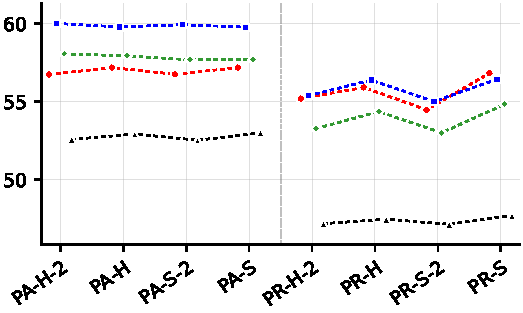
\includegraphics[width=\linewidth]{fig_rf_viruspseaac_pa_micro_f1_pa.pdf}\\\scriptsize micro-$f_1$ (\ref{eq:microf1}) ($\uparrow$)\end{minipage} \\[8pt]
\begin{minipage}{0.40\textwidth}\centering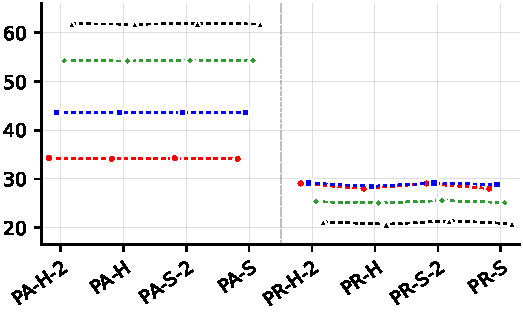
\includegraphics[width=\linewidth]{fig_rf_viruspseaac_pa_aabs.pdf}\\\scriptsize AABS (\ref{eq:aabs}) ($\downarrow$)\end{minipage} \\[8pt]
\begin{minipage}{0.40\textwidth}\centering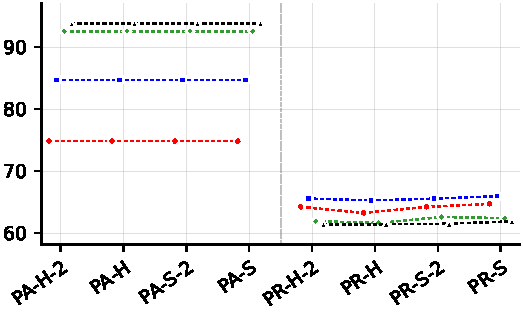
\includegraphics[width=\linewidth]{fig_rf_viruspseaac_pa_abs.pdf}\\\scriptsize ABS (\ref{eq:abs}) ($\downarrow$)\end{minipage} \\[8pt]
\end{tabular}
\caption{(Table G9) VirusPseAAC --- average scores (in \%, $y$-axis) over $5\times 5$ cross-validation folds, plotted against the classifiers ($x$-axis): partial-order predictors (PA-H-2, PA-H, PA-S-2, PA-S) and preorder predictors (PR-H-2, PR-H, PR-S-2, PR-S). Results are color-coded with respect to the noisy level $\alpha$ as follows: \textcolor[HTML]{FF0000}{$\alpha = 0.0$}, \textcolor[HTML]{0000FF}{$\alpha = 0.1$}, \textcolor[HTML]{339933}{$\alpha = 0.2$} and \textcolor[HTML]{000000}{$\alpha = 0.3$}.}
\label{tab:paperapp_g9_rf_pa_g1}
\end{table}

\FloatBarrier

\subsection{Abstention overview: aggregate trends}\label{sec:abstain_overview}
\paragraph{Purpose.} This compact section shows the headline abstention-vs-standard-MLC trend across noise levels, averaged over all datasets, for both base learners (RF, LGBM) and both retained quality metrics ($f_1$, Jaccard). Use it as a quick visual summary before diving into the detailed per-method / per-dataset figures in Section~\ref{sec:abstain_vs_mlc}.

\paragraph{How to read.} In each panel: blue bar = standard MLC (no abstention) on its native quality metric; coloured bar = with-abstention quality on retained labels. Green ``$+x.y$'' label = score-point gain of abstention over the standard-MLC bar of the same method. The four sub-panels per figure correspond to $\alpha\in\{0.0, 0.1, 0.2, 0.3\}$.

\begin{figure}[!htbp]
\centering
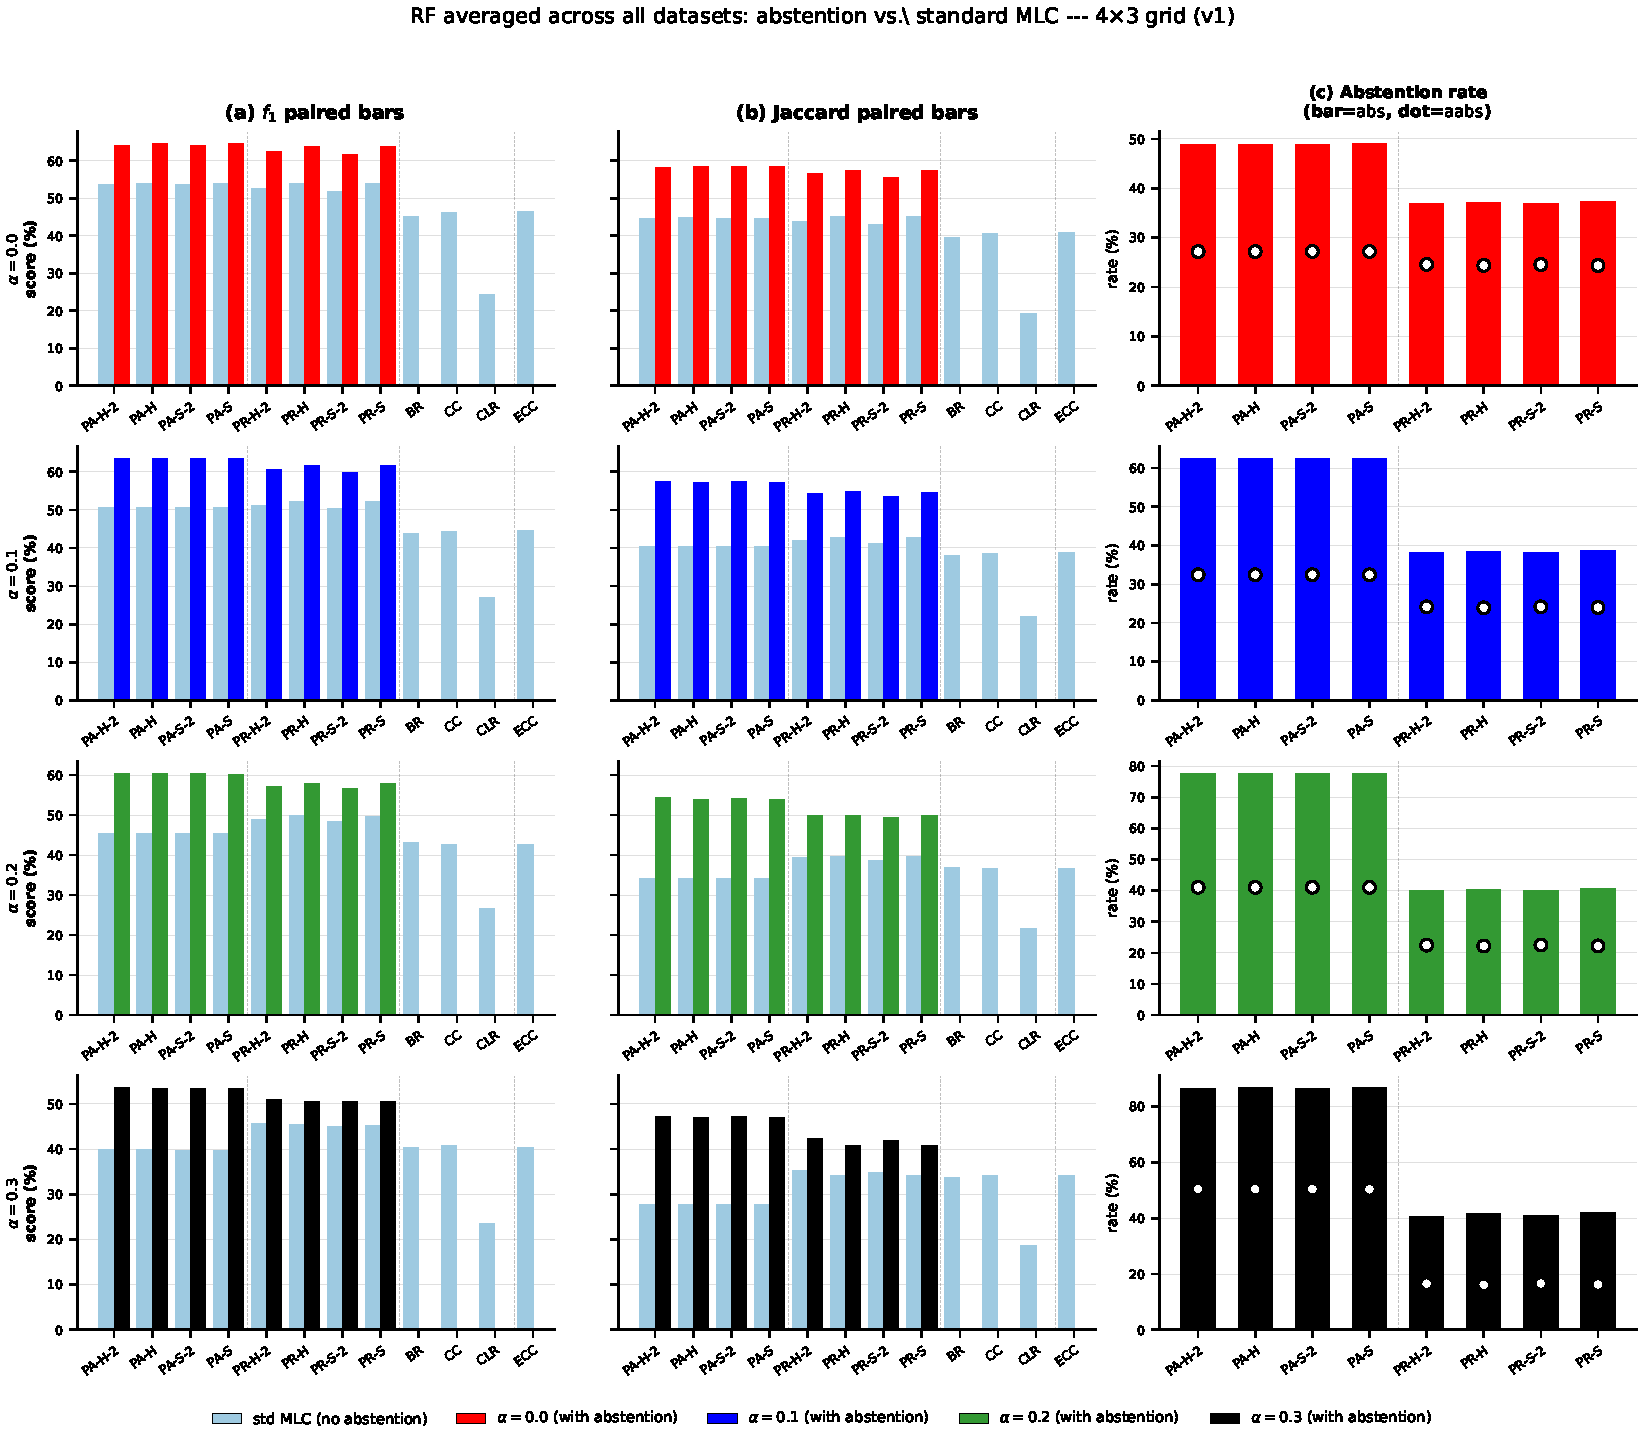
\includegraphics[width=\linewidth]{fig_rf_abstain_aggregate_summary_grid.pdf}
\caption{RF averaged across all datasets, $4\times 3$ grid (rows $=\alpha$, cols $=$ $f_1$ / Jaccard / abstention rate) --- (version~1) all 12 methods on the $x$-axis (PA + PR + baselines BR/CC/CLR/ECC); baselines plot only the std-MLC bar since they cannot abstain. Light blue $=$ standard MLC, $\alpha$-coloured $=$ with-abstention; in (c), bar $=$ \texttt{abs} (instance-level), dot $=$ \texttt{aabs} (per-cell). Color = $\alpha\in\{0.0, 0.1, 0.2, 0.3\}$.}
\label{fig:abstain_summary_rf_v1}
\end{figure}

\begin{figure}[!htbp]
\centering
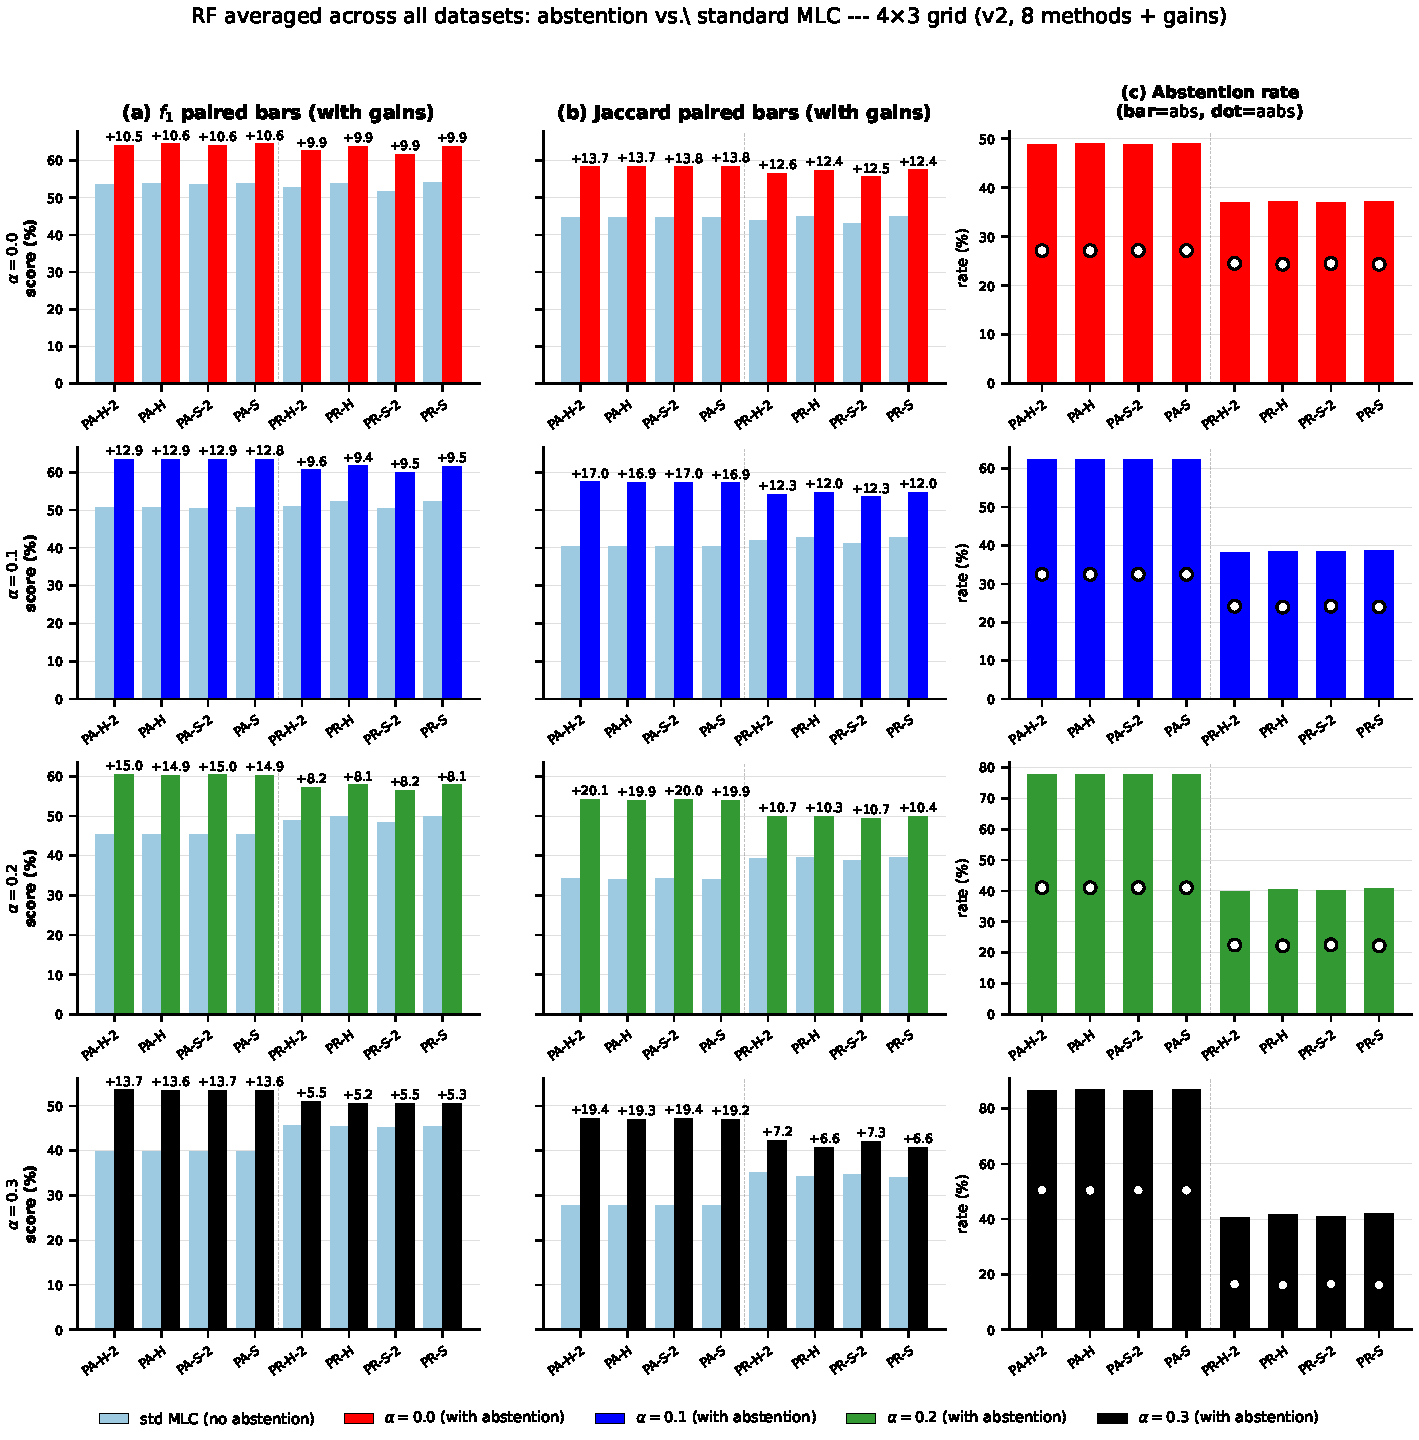
\includegraphics[width=\linewidth]{fig_rf_abstain_aggregate_summary_grid_v2.pdf}
\caption{RF averaged across all datasets, $4\times 3$ grid (rows $=\alpha$, cols $=$ $f_1$ / Jaccard / abstention rate) --- (version~2) only the 8 PA/PR methods that can abstain; gain labels $+x.y$ printed above each with-abstention bar so the score-point benefit over the std-MLC bar at the same method is visible at a glance. Same colour / layout conventions as version~1. Color = $\alpha\in\{0.0, 0.1, 0.2, 0.3\}$.}
\label{fig:abstain_summary_rf_v2}
\end{figure}

\begin{figure}[!htbp]
\centering
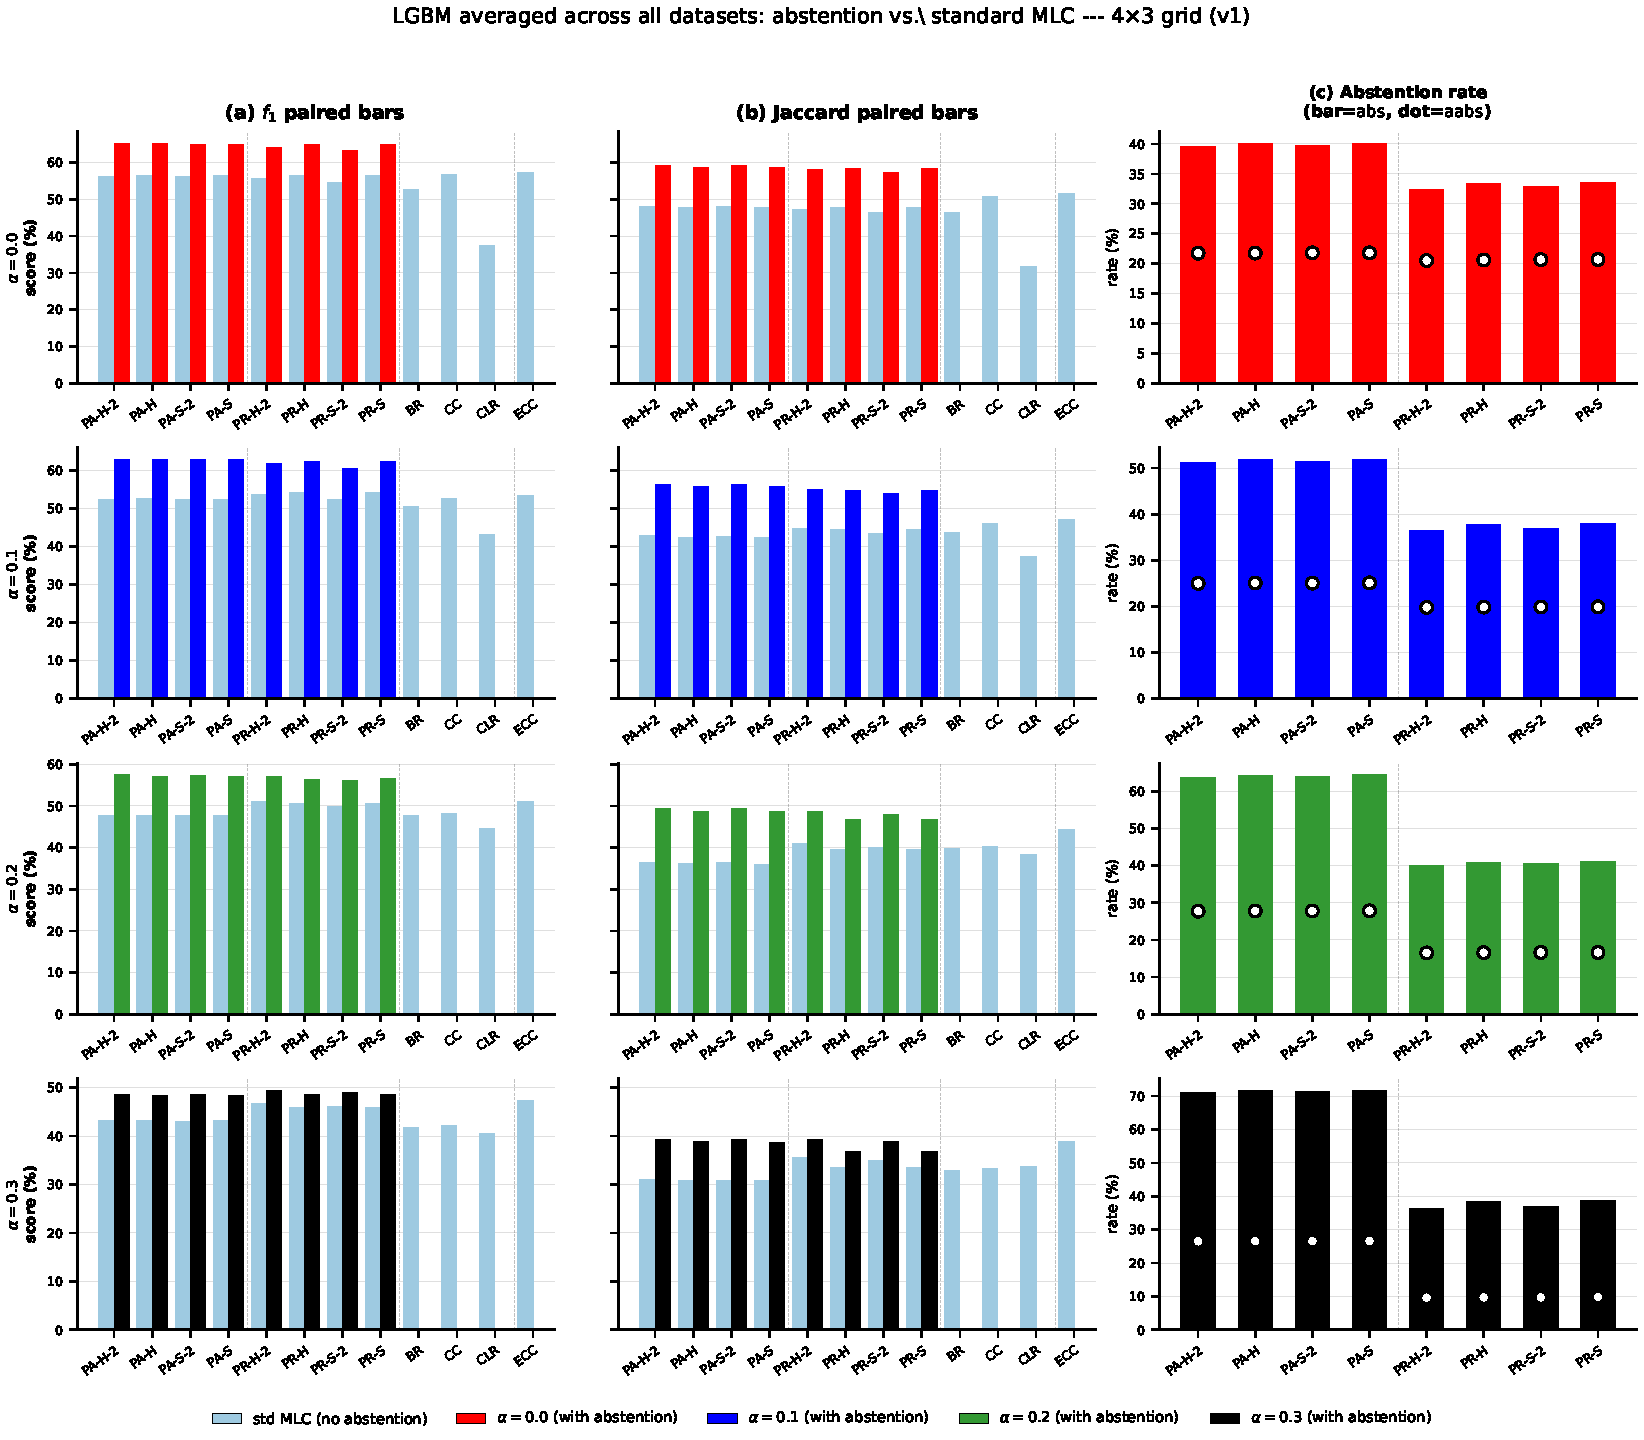
\includegraphics[width=\linewidth]{fig_lgbm_abstain_aggregate_summary_grid.pdf}
\caption{LGBM averaged across all datasets, $4\times 3$ grid (rows $=\alpha$, cols $=$ $f_1$ / Jaccard / abstention rate) --- (version~1) all 12 methods on the $x$-axis (PA + PR + baselines BR/CC/CLR/ECC); baselines plot only the std-MLC bar since they cannot abstain. Light blue $=$ standard MLC, $\alpha$-coloured $=$ with-abstention; in (c), bar $=$ \texttt{abs} (instance-level), dot $=$ \texttt{aabs} (per-cell). Color = $\alpha\in\{0.0, 0.1, 0.2, 0.3\}$.}
\label{fig:abstain_summary_lgbm_v1}
\end{figure}

\begin{figure}[!htbp]
\centering
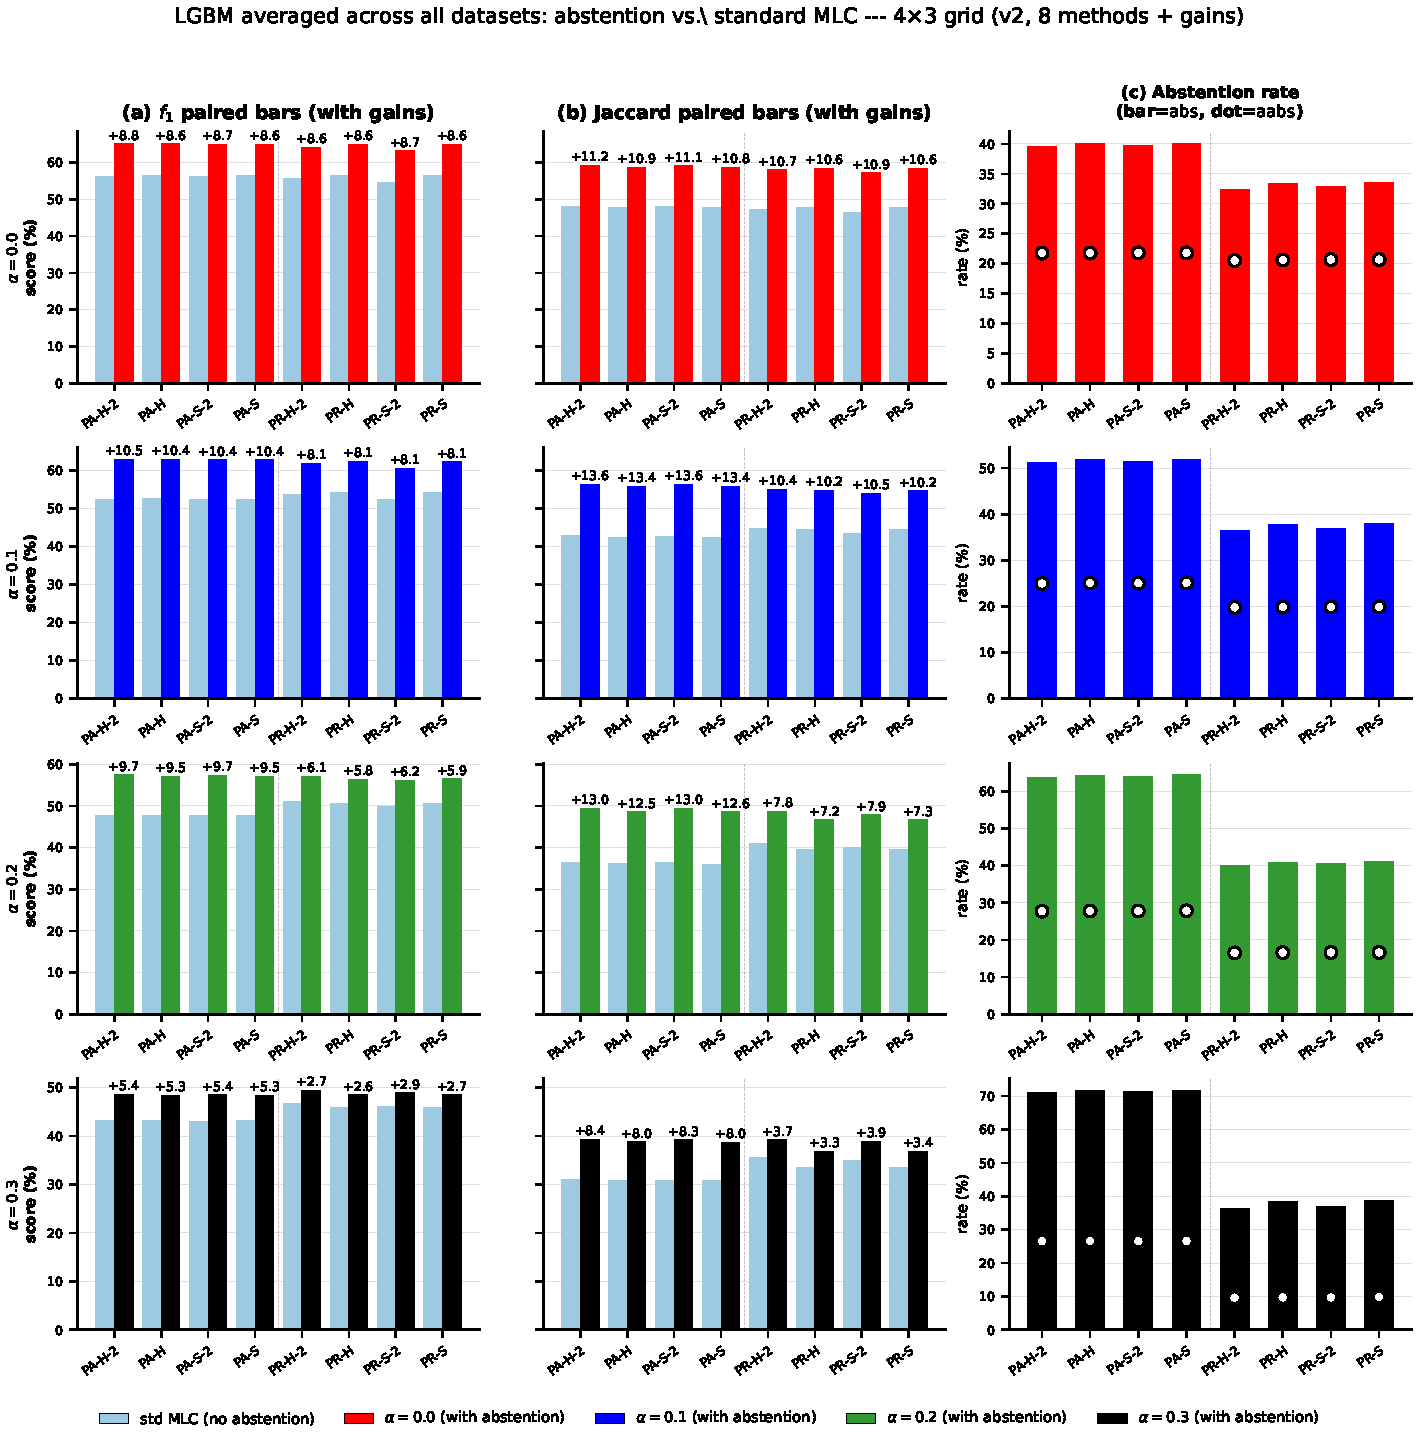
\includegraphics[width=\linewidth]{fig_lgbm_abstain_aggregate_summary_grid_v2.pdf}
\caption{LGBM averaged across all datasets, $4\times 3$ grid (rows $=\alpha$, cols $=$ $f_1$ / Jaccard / abstention rate) --- (version~2) only the 8 PA/PR methods that can abstain; gain labels $+x.y$ printed above each with-abstention bar so the score-point benefit over the std-MLC bar at the same method is visible at a glance. Same colour / layout conventions as version~1. Color = $\alpha\in\{0.0, 0.1, 0.2, 0.3\}$.}
\label{fig:abstain_summary_lgbm_v2}
\end{figure}

\FloatBarrier
\clearpage

\clearpage

\FloatBarrier

\end{document}
